\section{Tests écoute, suite et fin }

Tous les  tests d'écoute qui n'ont pas été mentionnés au chapitre précédent d'analyse  se trouvent 
répertoriés
en deux groupes. Les résultats de leurs analyses se trouvent sous la Figure  6.1.
Néanmoins, nous pouvons observer les modifications de l'écoute sans ou avec musicothérapie.
Le rapport entre la courbe aérienne (bleue) et la courbe osseuse (rouge) est facilement visible, ainsi que 
les pics, scotomes ou irrégularités représentant les tensions présentes et sous-jacentes.
 \subsection*{Groupe contrôle: GC  et Groupe musico: GM}
 
% \textbf { Patient F.:}
  \begin{figure}[th]
 	\centering
 	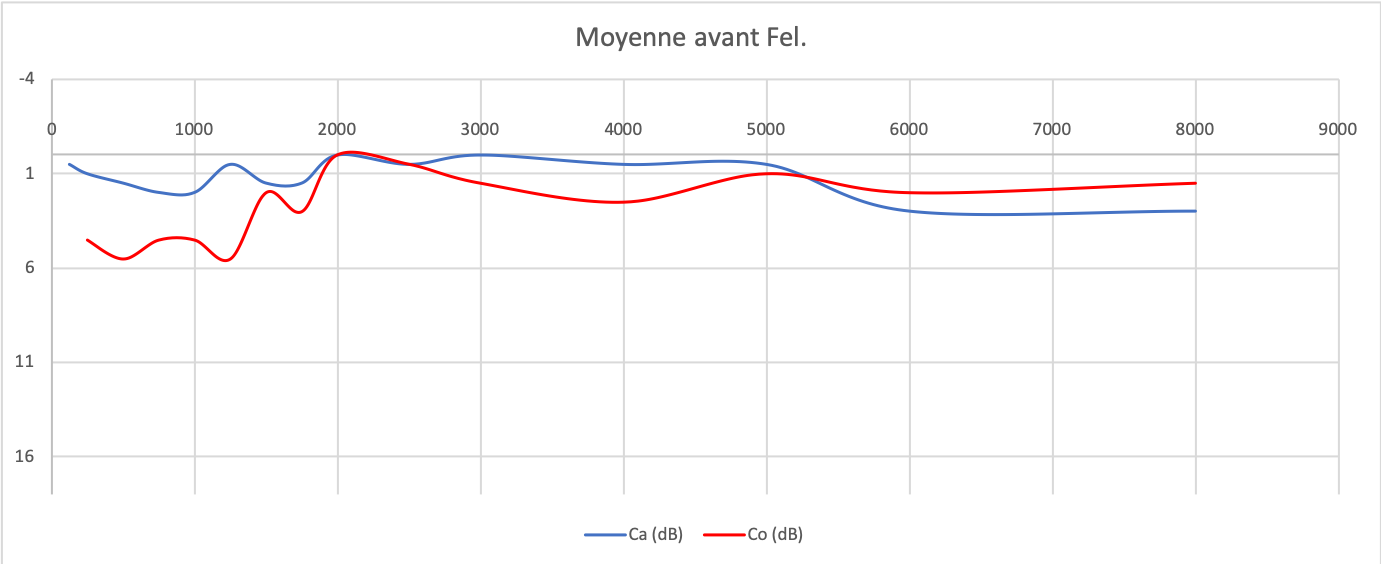
\includegraphics[width=0.7\linewidth]{images/graphiques/moyavFEL.png}
 	\caption[GC: Patient Fe: 1° test]{GC: Premier test Fe}
 \end{figure}
 \begin{figure}[th]
 	\centering
 	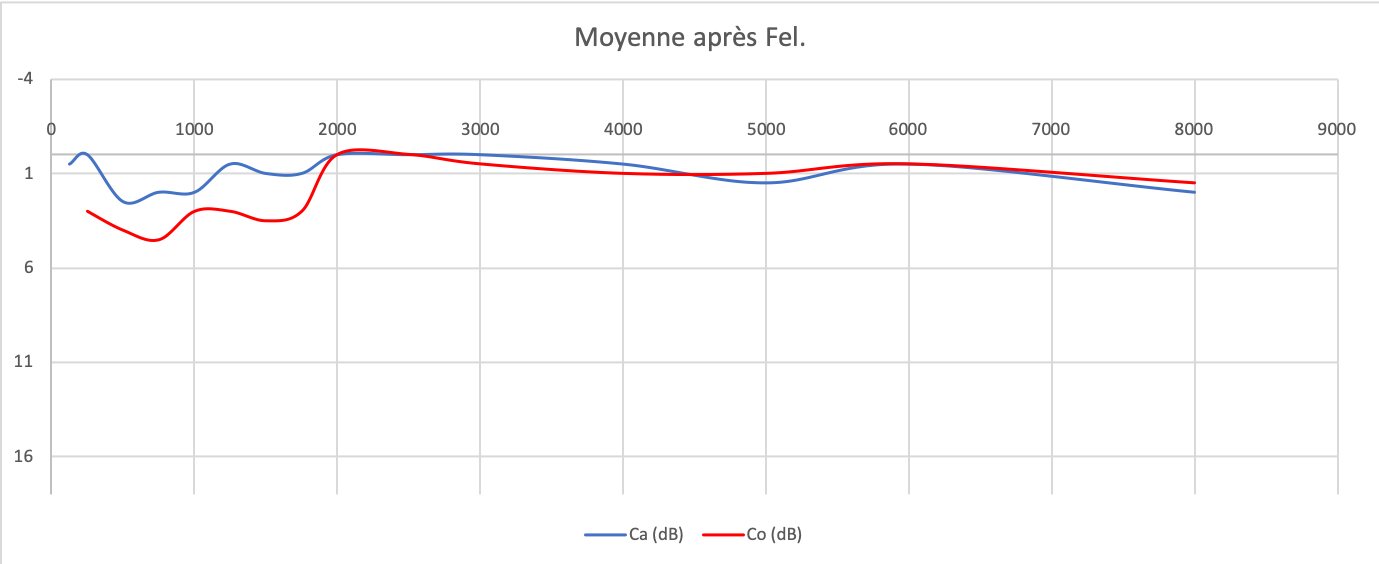
\includegraphics[width=0.7\linewidth]{images/graphiques/moyaprFEL.png}
 	\caption[GC: Patient Fe: 2° test]{GC: Deuxième test Fe}
 \end{figure}
 
% \clearpage
 
  %\paragraph
 %\textbf{ Patient L.:}
 \begin{figure}[th]
 	\centering
 	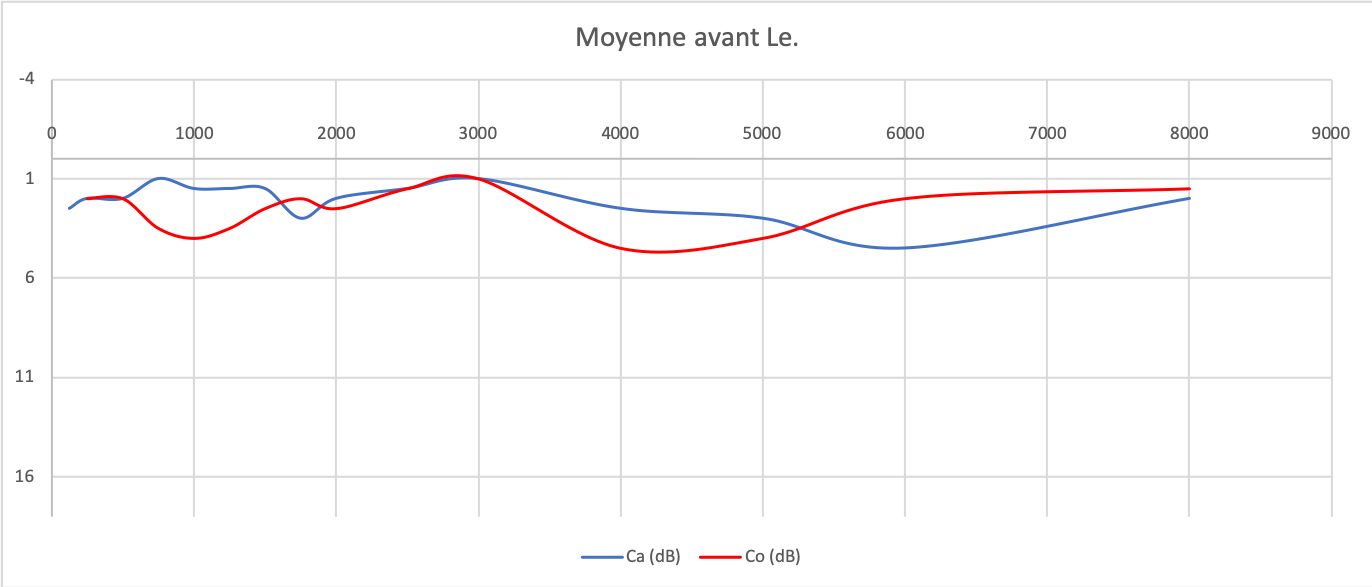
\includegraphics[width=0.7\linewidth]{images/graphiques/moyavLE.png}
 	\caption[GC: Patient Le : 1° test]{GC: Premier test Le}
 	\label{fig:moyavle}
 \end{figure}




  \begin{figure}[th]
 	\centering
 	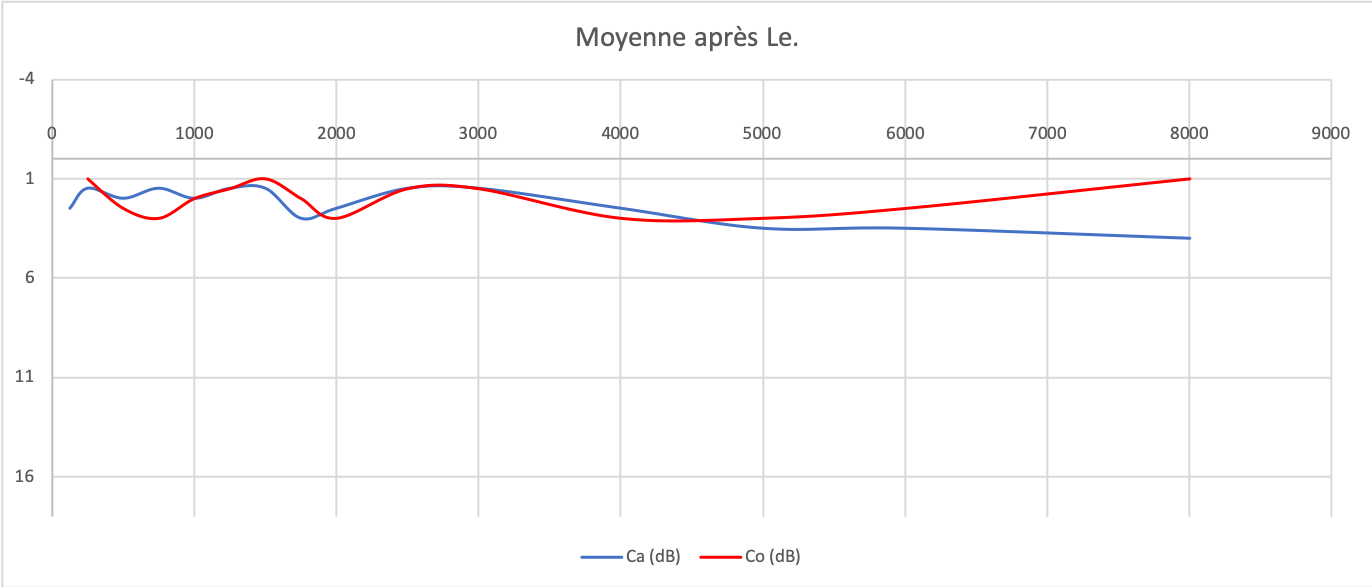
\includegraphics[width=0.7\linewidth]{images/graphiques/moyaprLE.png}
 	\caption[GC: Patient Le : 2° test]{GC: Deuxième test Le}
 	\label{fig:moyaprle}
 \end{figure}
 %\paragraph
 %\textbf{Patient MAI: 
  \begin{figure}[th]
 	\centering
 	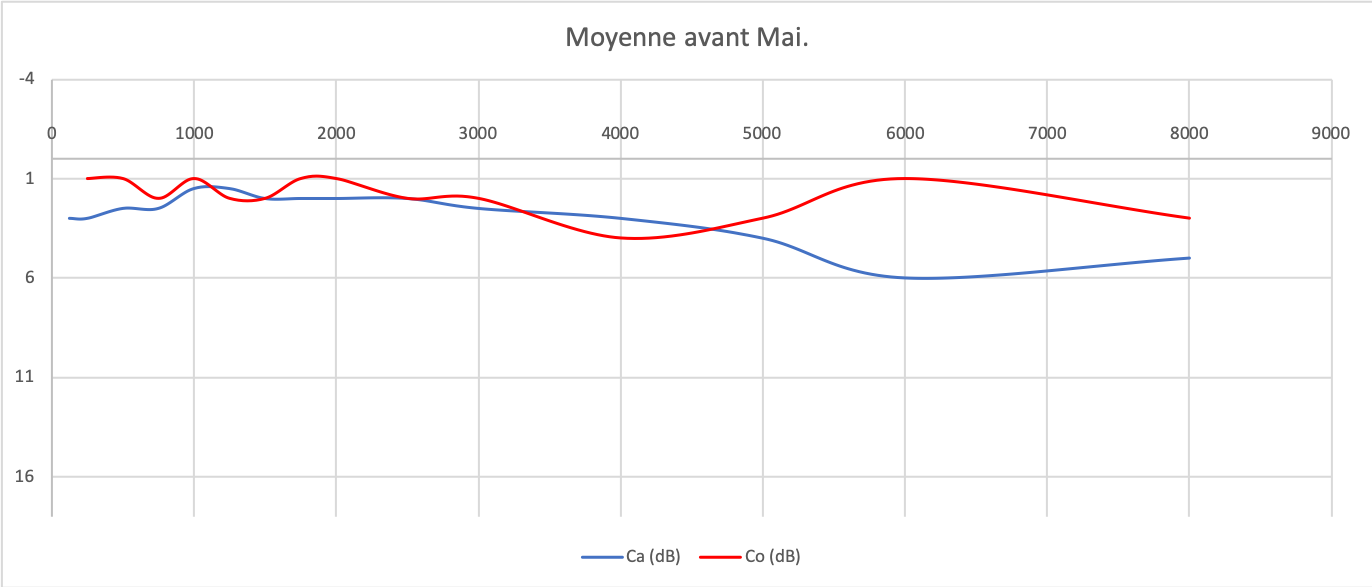
\includegraphics[width=0.7\linewidth]{images/graphiques/moyavMAI}
 	\caption[GC: Patient Mai : 1° test]{GC: Premier test Mai}
 	\label{fig:moyavmai}
 	 \end{figure}
  
  \begin{figure}[th]
 	\centering
 	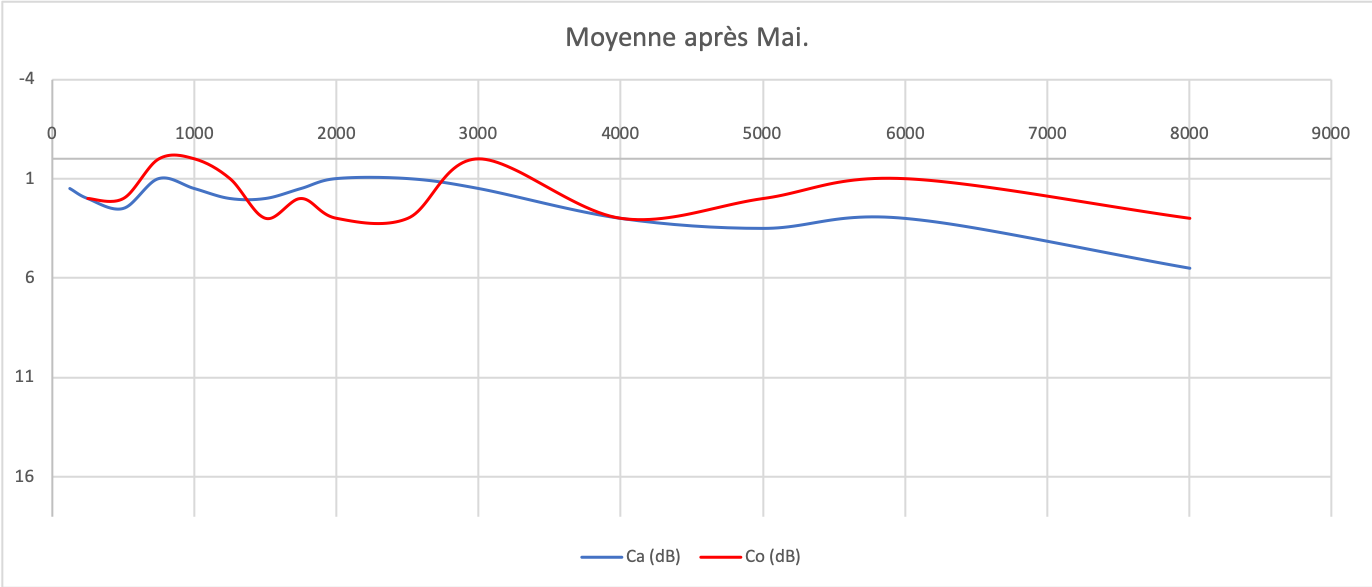
\includegraphics[width=0.7\linewidth]{images/graphiques/moyaprMAI}
 	\caption[GC: Patient Mai: 2° test]{GC: Deuxième test Mai}
 	\label{fig:moyaprmai}
 \end{figure}
 % \paragraph
% {Patient HU:}


% \clearpage
 \begin{figure}[th]
 	\centering
 	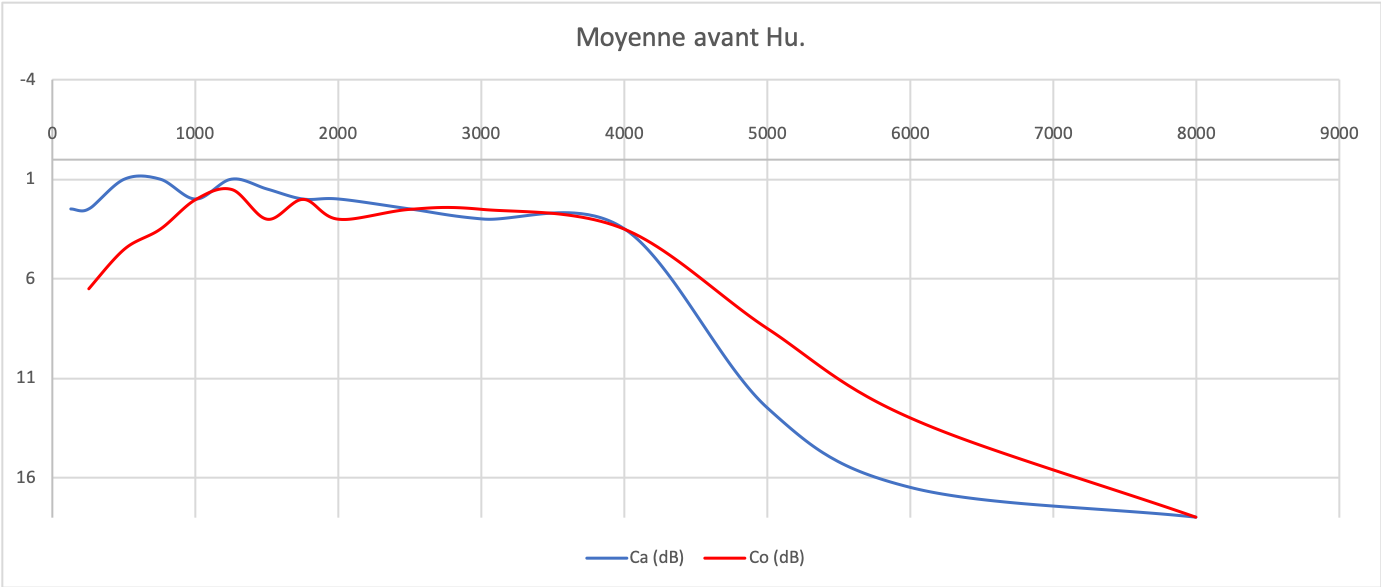
\includegraphics[width=0.7\linewidth]{images/graphiques/moyavHU}
 	\caption[GC: Patient Hu : 1° test]{GC: Premier test Hu}
 	\label{fig:moyavhu}
 \end{figure}



  \begin{figure}[th]
 	\centering
 	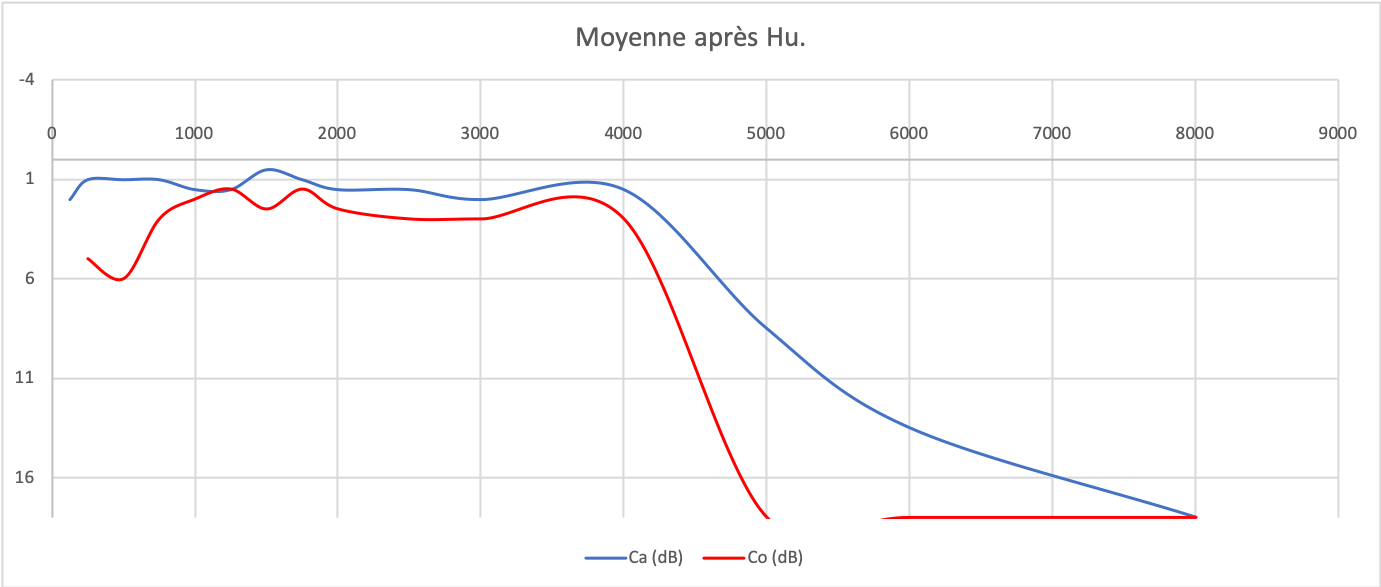
\includegraphics[width=0.7\linewidth]{images/graphiques/moyaprHU}
 	\caption[GC: Patient Hu : 2° test]{GC: Deuxième test Hu}
 	\label{fig:moyaprhu}
 \end{figure}
 
 
 
 
 % \section{Groupe musicothérapie}
% \paragraph{ Patients musico}
 % \clearpage
 
 \begin{figure}[th]
 	\centering
 	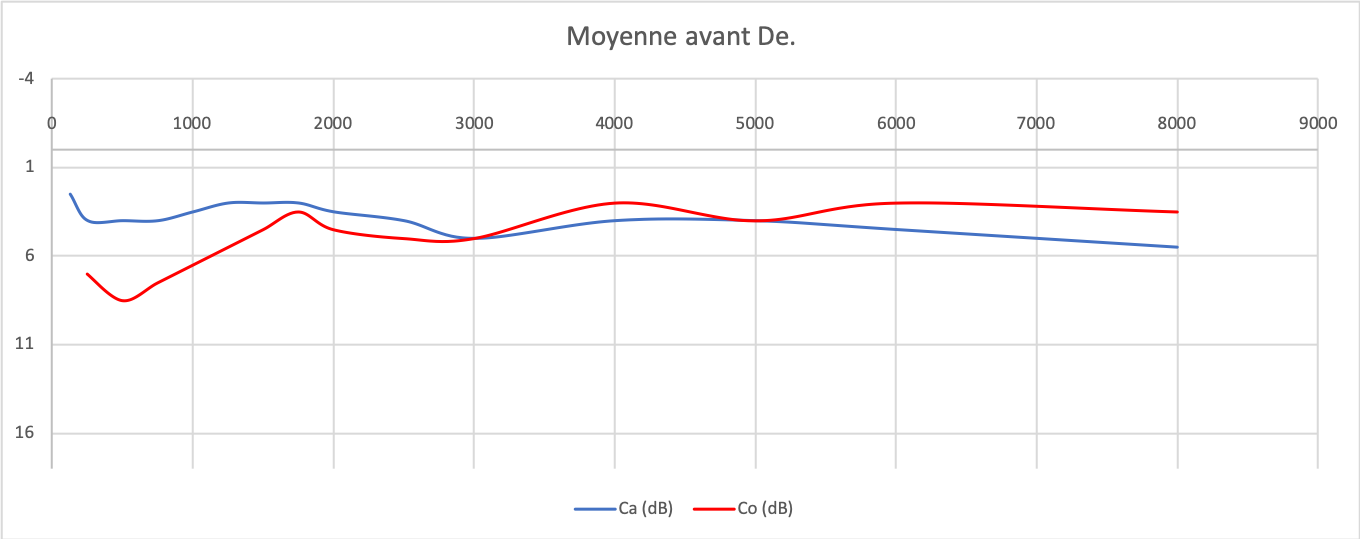
\includegraphics[width=0.7\linewidth]{images/graphiques/moyavDE.png}
 	\caption[GM: Patient De : 1° test]{GM: Premier test De}
 	\label{fig:moyavde}
 \end{figure}
 
 
 \begin{figure}[th]
 	\centering
 	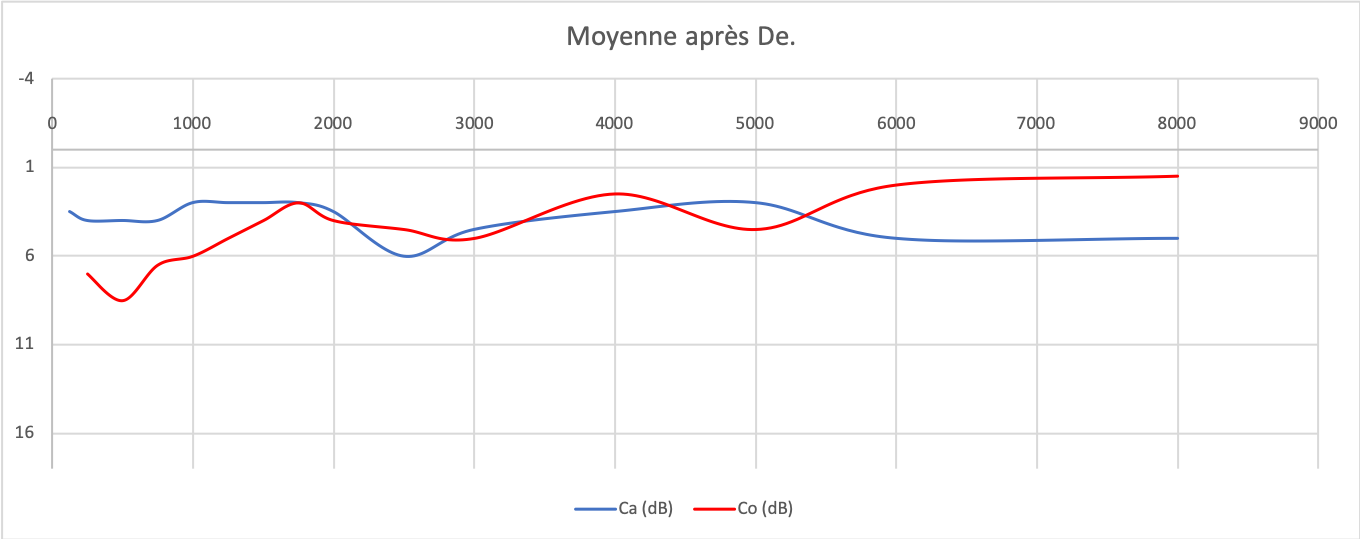
\includegraphics[width=0.7\linewidth]{images/graphiques/moyaprDE}
 	\caption[GM: Patient De : 2° test]{GM: Second test De}
 	\label{fig:moyaprde}
 \end{figure}
 
 
 %\paragraph{ Patient MU:}
 
 
 \begin{figure}[th]
 	\centering
 	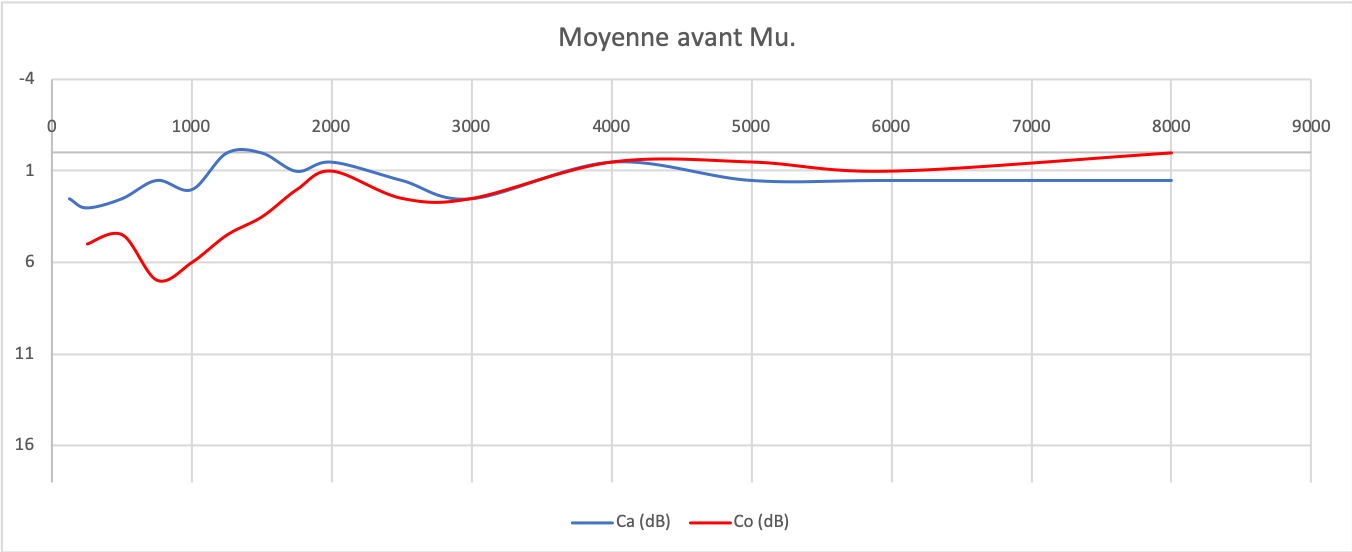
\includegraphics[width=0.7\linewidth]{images/graphiques/moyavMU.png}
 	\caption[GM: Patient Mu : 1° test]{GM: Premier test Mu}
 	\label{fig:moyavmu}
 \end{figure}
 
 
 \begin{figure}[th]
 	\centering
 	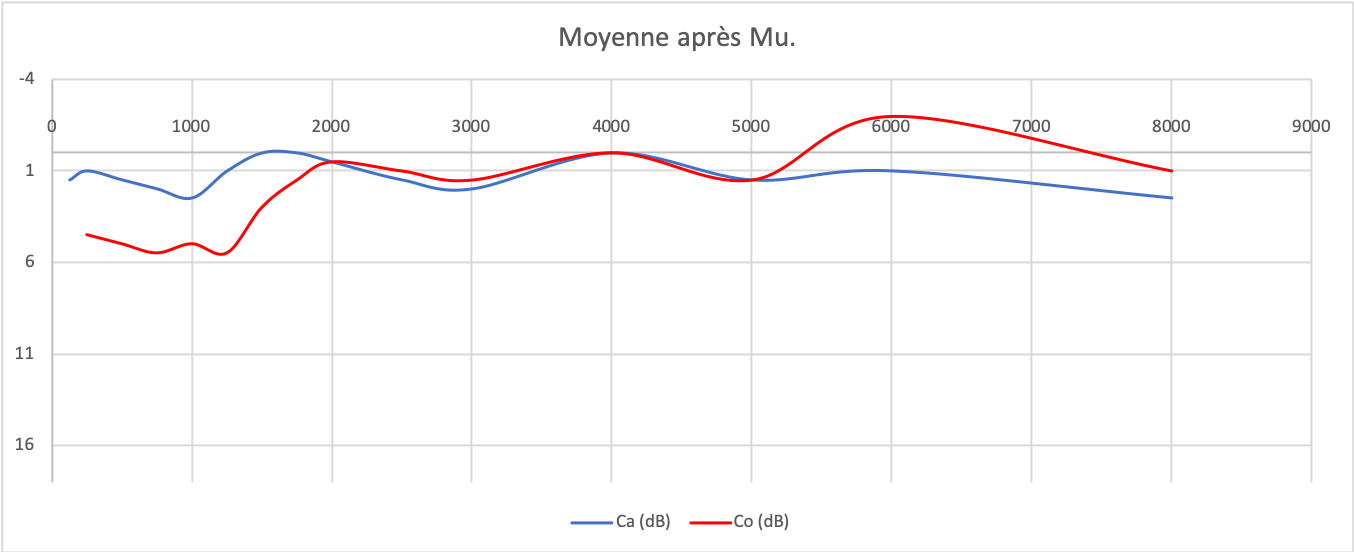
\includegraphics[width=0.7\linewidth]{images/graphiques/moyaprMU}
 	\caption[GM: Patient Mu : 2° test]{GM: Second test Mu}
 	\label{fig:moyaprmu}
 \end{figure}
% \clearpage
% Analyse d'un test d'écoute GM:
% \paragraph{D. Patient K.:}
 
% (pas de WOQOL fin de séjour)
 
 \begin{figure}[th]
 	\centering
 	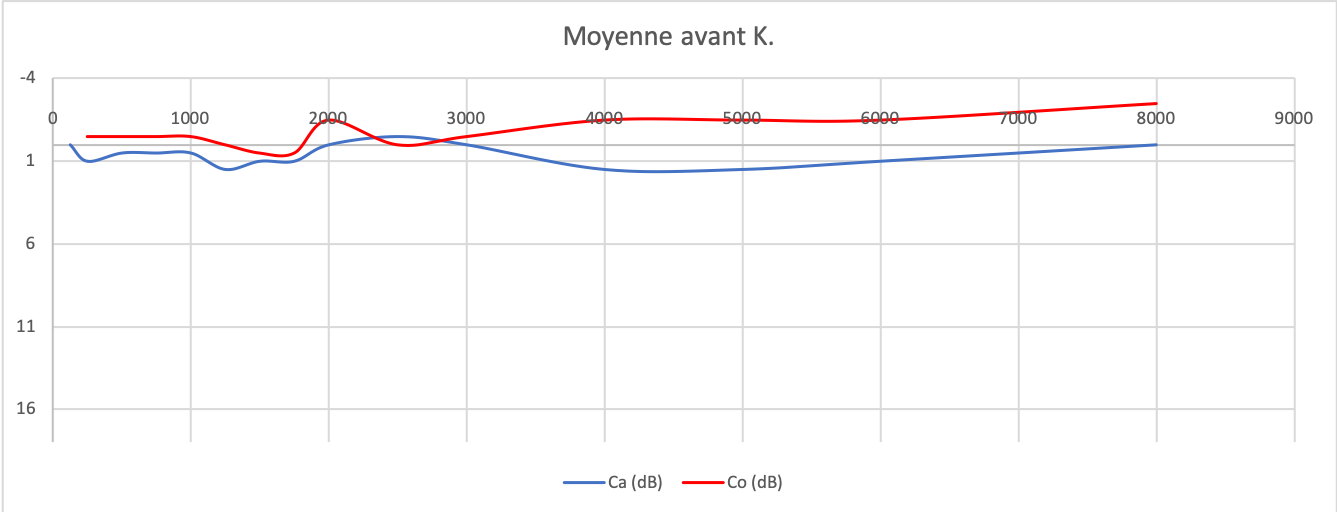
\includegraphics[width=0.7\linewidth]{images/graphiques/kad_pre.png}
 	\caption[GM: Patient K. . 1° test]{GM: Premier test K.}
 	
 	
 \end{figure}
 
 
 \begin{figure}[th]
 	\centering
 	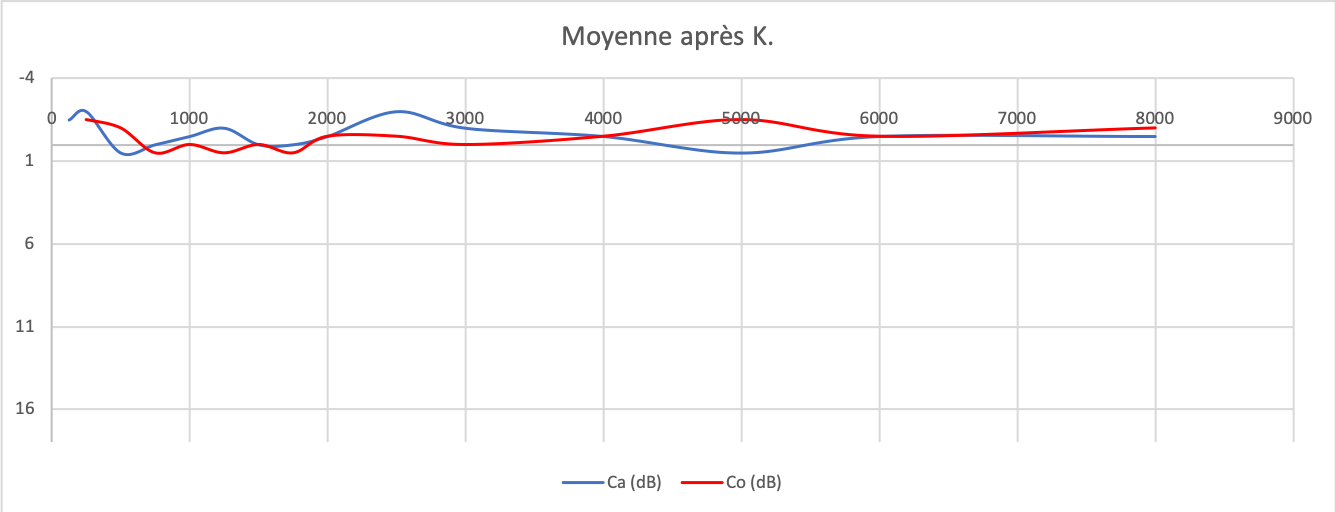
\includegraphics[width=0.7\linewidth]{images/graphiques/kad_post.png}
 	\caption[GM: Patient K. : 2° test]{GM: Second test K.}
 	
 \end{figure}



% \begin{enumerate}
 	
 %	\item : c.a.: redressement important: +
 	
 %	\item : c.o.: rapprochement et relèvement des seuils: +
 %	\item : croisements: 1/7 :  -
 	
 %\end{enumerate}
 
% \textbf{ Résultat:  + + -       : ``+''}
 %\textbf{ Equilibre ?
 %	questions : courbe: y a-t-il une modification en aérien et en osseux? si oui: +/ si  non: -
%              si modification, elle est équilibrée par la valeur des seuils       seuils diminuent-ils? oui : + : se 
%              relèvent-ils?
%                                 augmentent? non : - : 
%                                 
                                 
  %                                est-ce que ça va dans le bon sens? }
  
  
   \chapter{Résultats}
   Nous avons convertis les résultats finaux du test d'écoute et du questionnaire obtenus de façon à en 
   permettre la comparaison graphique et quantitative dans le cas des deux groupes (GM,GC).
   \\
   L'analyse comparative des résultats révèle une amélioration post traitement 
   du test d'écoute corrélée au questionnaire WHOQOL pour le groupe ayant suivi la musicothérapie. En 
   revanche, dans le groupe de contrôle il n'a pas été constaté d'amélioration post traitement. Les 
   séances de  
   musicothérapie semblent  ainsi avoir 
   eu un impact favorable dans la transformation de l'écoute, selon les normes dont nous avons parlé 
   avant. Cet impact semble également être corrélé avec une amélioration de la santé psychique des 
   patients, comme le WHOQOL le démontre. Nous allons observer ces résultats grâce aux deux 
   graphiques représentés par  les Fig. 6.1. et Fig. 6. 2.
 
 
    \textbf{ Synthèse  des résultats  des tests d'écoute Tomatis et des réponses au questionnaire 
    WHOQOL}
     L'ensemble de tous les résultats se trouve réuni et résumé
    aux Fig. 6.1. et Fig. 6.2.
    \begin{figure}
    	\centering
    	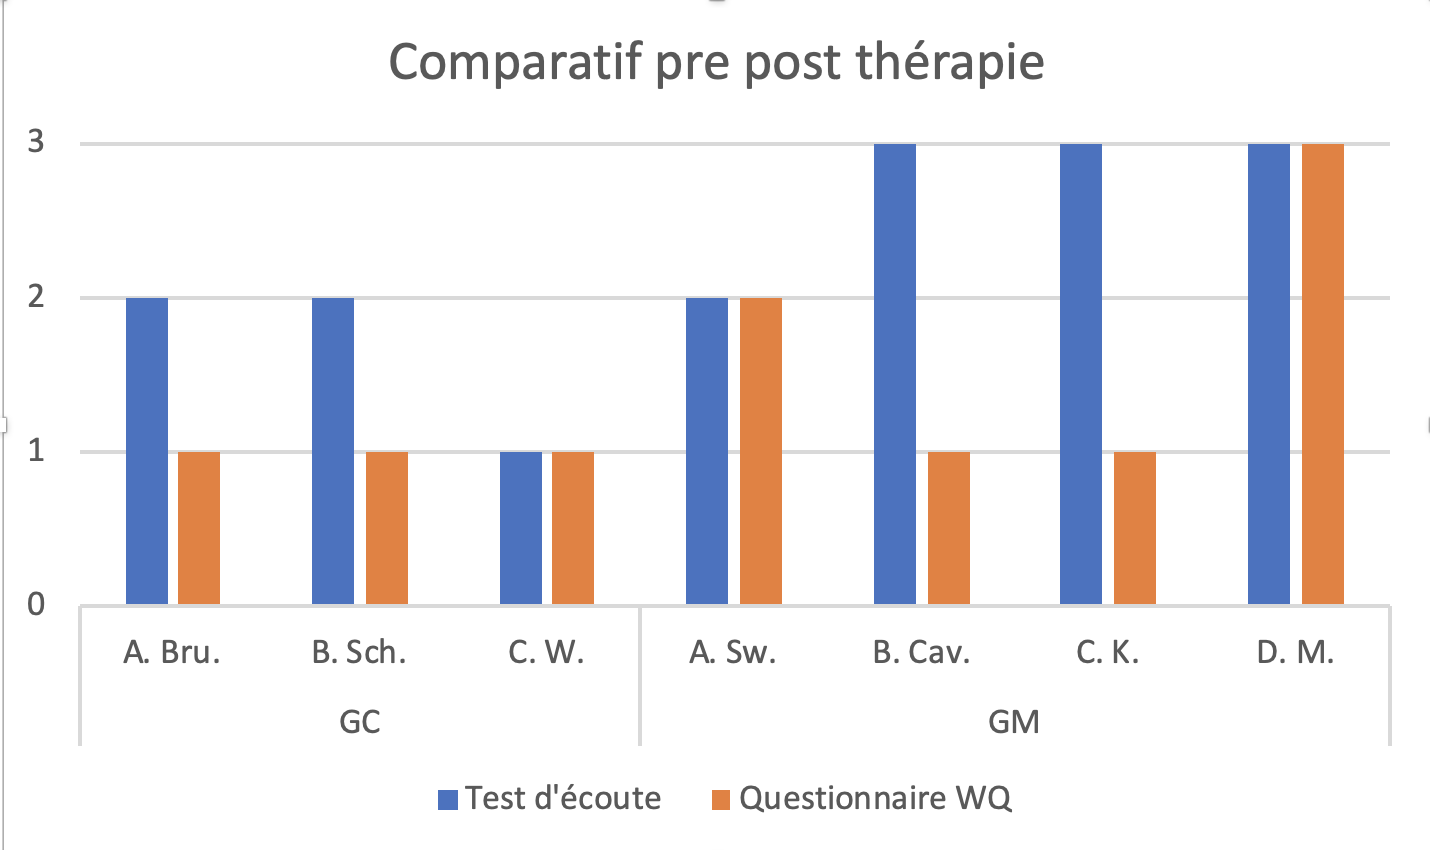
\includegraphics[width=0.7\columnwidth]{images/graphiques/comparatifWQecoute.png}
    	\caption[Comparatif résultats pré/post]{Comparatif des résultats entre WHOQOL et test d'écoute de  
    	GM et GC.}
    \end{figure}
    \clearpage
    La colonne bleue représente le résultat final 
    du test d'écoute et l'orange celle du questionnaire : les deux sont mis en parallèle 
    pour l'évaluation de leur correspondance. Les chiffres de 1 à 3 (-/=/+)représentent les degrés 
    d'amélioration, le 1 
    correspondant à une absence de changement.
    \\ 
    Les cas les plus probants attestant une corrélation entre le test d'écoute et le WHOQOL sont les 
    suivants: 
  \\
  Le patient M ( GM ) en est le meilleur exemple, avec une amélioration nette (3) tant sur le point 
  de la capacité d'écoute que sur le WHOQOL.
   \\
  Le patient Sw démontre également ce lien, néanmoins en degré moindre (2)
   \\
 %Les autres patients de GM (sans résultats WQ) attestent d'un résultat positif de la faculté d'écoute 
% sauf pour  Mu.  
Le patient F (GC) démontre une amélioration nette (3) tant sur le point 
 de la capacité d'écoute que sur le WHOQOL similaire à M.
 % Le patient W a démontré une 
% transformation de l'écoute sans éq
  Nous pouvons supposer dans ce cas l'illustration de  l'effet placebo et l'importance de  
  l'alliance 
  thérapeutique. Effectivement, se montrant extrêmement intéressé  par cette étude, le patient a 
  reçu de brèves explications 
  sur le possible impact des séances de musicothérapie; la réaction du patient 
  a été une écoute assidue de musique  pendant son séjour. Le résultat final est très positif au point de 
  vue du WHOQOL comme sur celui du test 
  d'écoute, nous pouvons le constater clairement  à la 
  Fig. 6.1 et 6.2.  En conclusion, dans ce cas particulier, les séances de musicothérapie n'ont eu aucune  
  influence directe sur 
  l'amélioration du ressenti de la qualité de vie ni sur la capacité d'écoute. Par contre, le contact 
  thérapeutique, loin de toute objectivité, a joué un rôle important.
  
  
  Sous forme de pourcentage, nous pouvons constater les mêmes résultats (positif, négatif et neutre) 
 selon leur fréquence: on constate ainsi une augmentation des résultats positifs du test d'écoute dans le 
 cas du groupe ayant suivi la musicothérapie ( 66,7\% vs 28,6\% ). 
 	 \\ 
 Quant aux réponses du questionnaire WHOQOL, nous constatons une équivalence entre positif et 
 négatif (50\%) pour GM et de faibles résultats positifs pour GC (28,6\% vs 71,5\%).
    
   \begin{itemize}
   	 \item Résultats pour le test d'écoute:
   	 \\ 
 GC: 
  \\
2 résultats positifs sur 7:       2/7 - 28,6\%
\\
3 résultats neutres sur 7:			3/7 - 42,9\%
 \\
 2 résultats négatifs sur 7:		2/7 - 28,6\%
 \\
GM:
  \\
 4 résultats positifs sur 6    :       4/6 - 66,7\%
  \\
  1 résultat neutre sur 6 : 			1/6 - 16,7\%
 \\  
  1 résultat négatif sur 6 : 		     1/6 - 16,7\%
 \\
%\part{title} 
  		    \item Réponses pour le questionnaire:    
 \\
 GC: 
 \\
 2 réponses positives sur 7:       2/7  - 28,6\%
 \\
 5 réponses négatives sur 7: 	5/7 - 71,5\%
 \\
 GM:
  \\
 1 réponse positive sur 2    :       1/2 - 50\%
   \\
   1 réponse neutre sur 2 : 			1/2 - 50\%
  		  \end{itemize}
  	  
  	  
% \begin{itemize} 
% \item \textbf{Groupe Contrôle:} 	          \textbf{ test d'écoute: ``=''   et    WQ: ``-'}


% \item \textbf{Groupe Musicothérapie:}     \textbf{test d'écoute: ``+''      et    WQ: ``+''}
%  \end{itemize}
  \begin{sidewaysfigure}
  	\centering
  	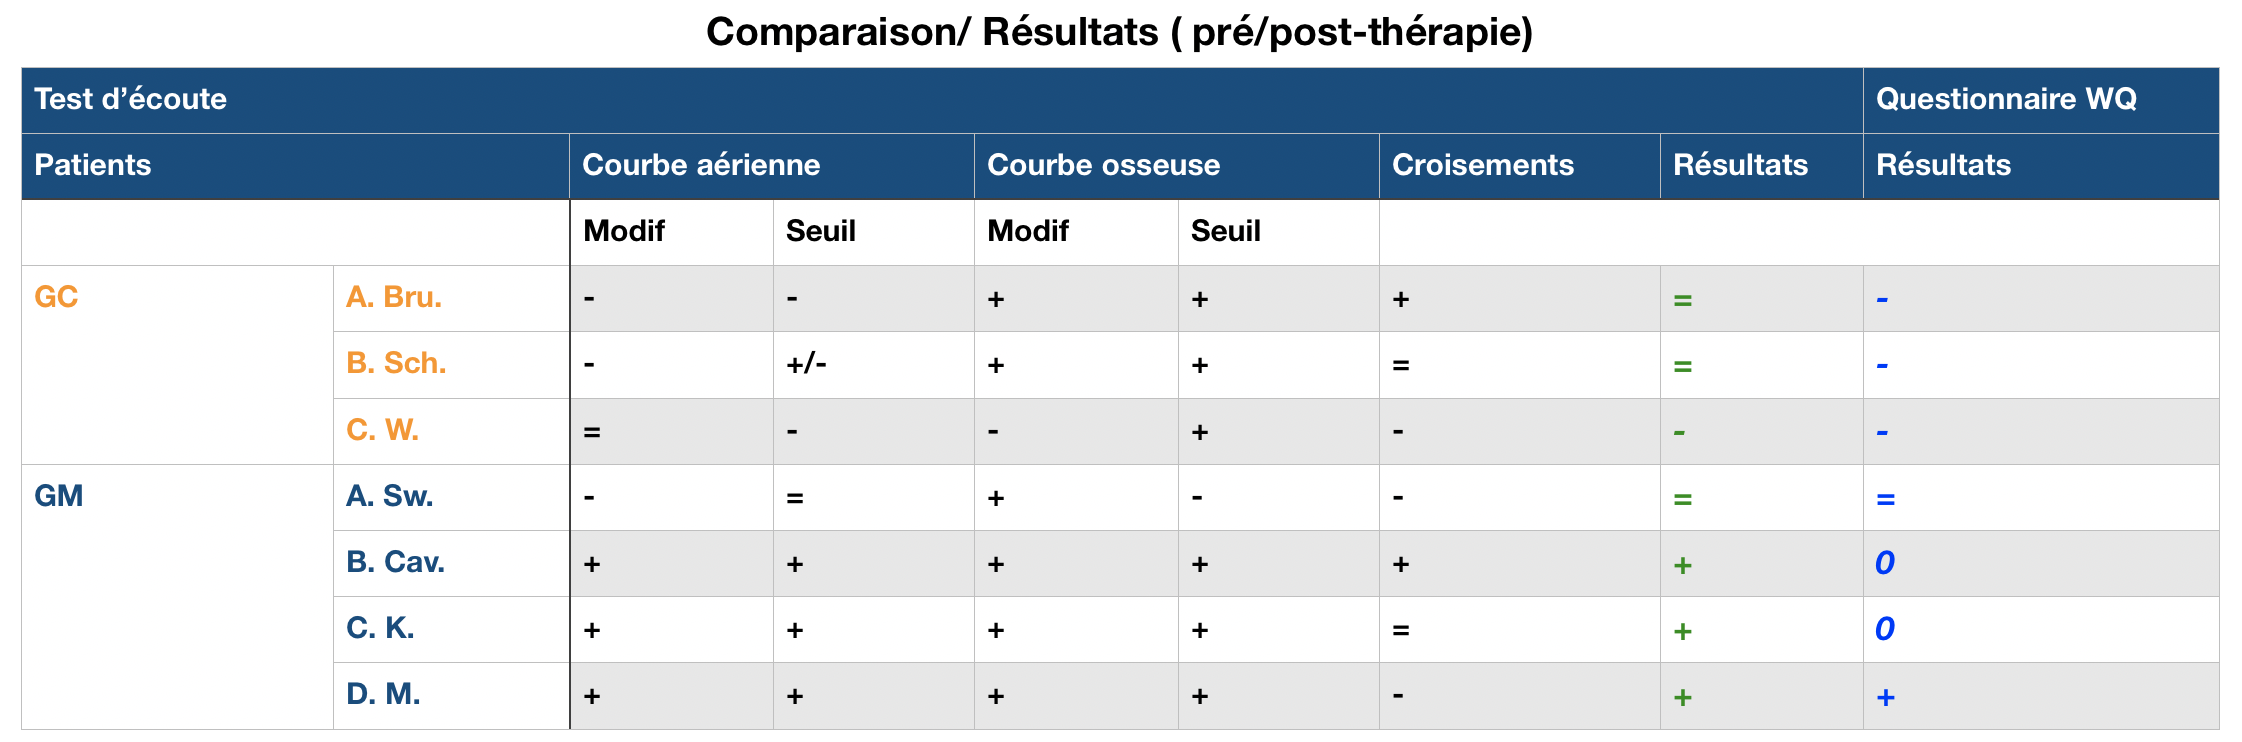
\includegraphics[width=0.7\columnwidth]{images/graphiques/comparaison_pre_post.png}
  	\caption[Résultats de la comparaison ( WHOQOL/ test écoute)]{Résultats de la comparaison ( 
  	WHOQOL/ test 
  	écoute)}
  	
  \end{sidewaysfigure}
   
%   \clearpage
  
  
\chapter{Discussion}
\label{Conclusions}

Notre étude s'est passée  en milieu psychiatrique, 
auprès de patients souffrants de troubles de l'humeur.
Elle a porté sur plusieurs observations: d'une part sur celle de la faculté d'écoute, révélée par un test 
d'écoute selon la méthode Tomatis, test effectué deux fois, en début et fin de thérapie.
% de l'état de la personne.
\\
D'autre part, elle a porté sur l'observation générale des séances individuelles en musicothérapie.
Et enfin, elle a porté sur la quantification du ressenti subjectif de la qualité de vie au moyen du 
questionnaire WHOQOL, effectué deux fois, en début et fin de séjour en clinique.


\paragraph{L'objectif de ce travail} a été de vérifier l'hypothèse suivante: 
	 la  mesure de la  transformation de la capacité d'écoute révèlerait  l'importance de l'impact  du 
	 traitement 
musicothérapeutique sur la capacité d'écoute.
Nos questions de recherche sont: 
\begin{itemize}
	\item Une musicothérapie ciblée sur l'écoute  est-elle en lien avec une modification de la qualité 
	d'écoute 
	mesurable par le test d'écoute Tomatis?
	\item La transformation de la capacité d'écoute est-elle  proportionnelle au changement 
	du sentiment de qualité de vie du patient?
\end{itemize}





  %\footnote{cité
 % par S.Aubert- Khalfa et al.: Yovell, Y.,
 %   Sackeim,H.A., Epstein, D.G.,Prudic, J., Devanand, D.P. McElhiney,
  %  M.C. Settembrino, J.M. Bruder, G.E., 1995. Hearing loss asymmetry in
  %  major depression.J.Neuropsychitr. Clin. Neurosci. 7, 82--89 / Journal of Affective Disorders 127
   % (2010) 170}

 L'axe principal a porté sur la comparaison de la faculté d'écoute des patients en conclusion d'un suivi 
 individuel en musicothérapie après trois semaines en cadre clinique.
 Le test d'écoute Tomatis\textsuperscript \textregistered  et le questionnaire WHOQOL sur la qualité de 
 vie 
 ont été les moyens 
 utilisés 
 pour synthétiser les différences. 
 Treize  patients, avec troubles de l'humeur, ont été assignés à deux groupes de recherche: 
 six au groupe
 musicothérapie (GM) et sept au groupe contrôle (GC).
  L'analyse comparative des résultats a révélé une modification positive et significative 
 de qualité d'écoute après musicothérapie 
 pour GM contrairement à GC, résultats correspondants à ceux recueillis par  %au ressenti subjectif 
 le questionnaire WHOQOL. 
 
 En conclusion, la musicothérapie a
 eu un impact positif autant sur la qualité d'écoute que sur la qualité de vie  du patient.
Une amélioration du tracé des courbes d'écoute allant dans la tendance d'une courbe harmonieuse en 
fin de séjour a corroboré une amélioration de la qualité d'écoute; cette dernière pouvant être 
possiblement corrélée avec une amélioration du ressenti du patient quant à sa qualité de vie, ressenti 
mesuré au moyen du test WHOQOL.

 La totalité des tests d'écoute et des questionnaires demeure toutefois 
 inférieure à ce qui avait été initialement planifié, et, en dépit d'une plus ample dimension statistique, ce 
 travail a avantagé plus les aspects qualitatifs que quantitatifs.
 
  \section{ L'impact des différences d'écoute }
 Notre intérêt s'est centré essentiellement sur l'analyse d'une
 	observation
 portant sur la transformation de la capacité d'écoute à l'aide de
 l'appareil test afin de répondre aux questions de recherche: 
  \begin{itemize}
       \item Une musicothérapie ciblée sur l'écoute  est-elle en lien avec une modification de la qualité 
       d'écoute 
       mesurable par le test d'écoute Tomatis?
          La capacité d'écoute est quantifiable  par le test d'écoute Tomatis.
  %nous avons pu l'observer.et  assister à sa
  %transformation. 
  S. Aubert -Khalfa et son équipe multidisciplinaire \autocite{affectiveDisorders} avaient déjà
  exploité le test Tomatis\textsuperscript \textregistered    sensible à la différence des
  seuils auditifs mais sans pré/post observation. Ils l'avaient fait sur une population
  dépressive avec stress post-traumatique et sur une autre, normale. De notre côté, nous avons choisi
  une population de même type de pathologie avec comparaison en fin de séjour.
  Notre étude est sans commune mesure avec celle-ci. Toutefois, 
  des résultats convergent puisque nous avons pu observer de manière générale  une transformation et 
  importante sensibilité des seuils auditifs dans les deux groupes. 
  
  
 	La modification de la capacité d'écoute observée est liée
 au traitement musicothérapeutique 
 % La capacité d'écoute est impactée par le traitement en musicothérapie. 
  puisque nous avons constaté une modification de la  
 sensibilité des 
 seuils auditifs du groupe de musicothérapie.
Le test de capacité d'écoute nous a permis de constater l'impact des différences  entre ceux qui ont 
bénéficié d'un 
 traitement en  musicothérapie et ceux qui n'en ont pas eu.
  \\
  Comme déjà évoqué à propos des trois zones du test, 
 dans l'accompagnement thérapeutique évolutif du patient,
 les transformations perceptives visibles sur
 le tracé sonore (le graphique des courbes) nous incitent à une modulation
 musicothérapeutique mieux adaptable et différemment ajustable.
 En se référant aux
 différentes zones, nous avons pu relever différentes pistes de travail dans le but de
 solliciter le patient plus précisément. 
 Si la courbe aérienne est restée
 totalement plate et non
 réactive par exemple en zone 2, nous avons recouru plus à l'expression verbale, en zone 1, plus aux 
 rythmes ou à l'improvisation en zone 3.
 D'autre part, ce test spécifique est un travail en soi en musicothérapie: on a remarqué  lors du 2° test en 
 fin de 
 thérapie, une attention particulièrement affinée sur la façon d'écouter,  attitude différente que celle lors 
 du 1° test.
  \\
  Nous pouvons considérer ainsi le test d'écoute comme complémentaire, se confirmant dans une 
  évaluation plus
 précise de l'utilisation d'outils variés, y compris au sujet du parcours effectué et à
 construire. Il peut être une aide en permettant  d'avoir des repères et une optique un peu différente dans 
 la façon d'aborder un travail en musicothérapie.
  \newline 
 
 %, en recourant à davantage  à la voix ou à l'improvisation,
 %plus qu'aux rythmes, à titre d'exemple.
 
 
 
 
 	\item La transformation de la capacité d'écoute est-elle  proportionnelle au changement 
 	du sentiment de qualité de vie du patient?
   Cette transformation de la capacité d'écoute peut être proportionnelle au changement du sentiment de 
   qualité de vie du patient puisqu'il existe une corrélation entre test de capacité d'écoute et questionnaire 
   WHOQOL.
 \newline 
     Pour le groupe de contrôle, il nous a
 apporté un autre regard avec des compléments d'informations au 
 questionnaire
 WHOQOL. Quoique l'ensemble des résultats avec le WHOQOL est
 négatif et neutre pour le
 test d'écoute, nous avons pu observer, grâce aux tests, une 
 courbe 
 aérienne
 sans modification mais une courbe osseuse plus
 particulièrement réactive. 
 %Nous allons y revenir lors de la discussion.
 Nous pouvons émettre l'hypothèse de   %déceler 
 la sous -- jacence 
 d'un mouvement interne qui se traduirait par 
 %une ébauche, 
 une amorce de
 processus intérieur,  quoique inconscient. Contrairement au ressenti éventuel du patient, il y  a, par un 
 autre biais, peut-être une 
 ébauche de sa transformation mise en lumière de façon originale  par sa capacité d'
 écoute. Le dialogue, lors de l'issue du test final, provoquera un autre 
 regard du patient sur lui-même.
  \newline 
 Conclusion: au cours de l'étude que nous avons mené, nous avons pu constater de manière générale, 
 qu'il existe des modification de la capacité d'écoute, indépendamment du groupe testé. On peut donc 
 supposer que le séjour clinique a un impact sur le patient d'un point de vue écoute.
 \newline 
 Néanmoins le temps de séjour des patients semble être trop court pour obtenir des résultats qualitatifs 
 et statistiquement significatifs. Il est tout de même intéressant de noter que durant le temps de séjour 
 relativement bref des patients, nous avons tout de même pu constater une amélioration substantielle 
 des courbes de capacité d'écoute, nous menant à nous interroger sur l'intérêt d'une thérapie plus 
 intensive, que ce soit en fréquence ou en durée. On pourrait également prendre en compte les 
 traitements médicamenteux que suivent chaque patient, traitements qui dans le domaine psychiatrique 
 ont une influence non négligeable sur la qualité de vie du patient, et donc possiblement comme nous 
 avons essayé de le montrer durant cette essai, un effet sur la capacité d'écoute de ces derniers.
 
 
  
 Réflexions:
  \\
 Le test d'écoute tout en n'étant pas un audiogramme,  peut  être aussi considéré comme un 
 outil de sensibilisation à certains problèmes de surdité. Il en est de même avec la détection de distorsion:
 pouvant être autant physiologique que psychologique. Le tympan va se tendre ou se 
 distendre 
 selon les problèmes rencontrés. Cette inter -- réactivité physique et psychique joue son rôle et a son 
 poids dans la compréhension du patient. Il donne un point de vue complémentaire.
  Les problèmes relevables dans la capacité d'écoute peuvent ainsi être  le reflet de la somatisation de 
 problèmes psychiques: 
 cette sorte de  "mise  à jour" par le test donne un éclairage différent sur le patient, cible ses points 
 faibles et aide 
 parfois lors de diagnostic difficile à cerner.
  \\
  Ceci nous amène à considérer  l'anamnèse et le bilan en musicothérapie.
 Il y a un temps qui
 précède
 l'amorçage de la thérapie et celui suivi de la thérapie elle-même.
 En réalité, ces aspects s'enchevêtrent à un point tel que
 l'utilisation du test peut assumer même un rôle musicothérapeutique, fournissant des
 renseignements immédiats à l'anamnèse sous forme de multiples
 aspects du son: l'émission du son de
 l'appareil vers le patient suscite une  réaction gestuelle.  Ces réponses  
 donnent des indices de réception %évitant toute confusion
 quelle que soit la langue utilisée, procédé non-verbal
 	spécifiquement axé sur le son, par conséquent  musicothérapeutique. 
 	D'autre part, lors du second test de capacité d'écoute, 
 
Ce test avec des sons purs peut apporter plus d'objectivité. Néanmoins, comme nous le fait remarquer 
Tomatis,
\enquote{l'influence des paramètres subjectifs en audiométrie ont été prouvés par les travaux de 
	l'Américain Ralph. F. Naunton}  \autocite [69]{tomatisoreilletvie}. Quoiqu'il existe ici cette différence 
entre 
test d'écoute et audiomètre,
%d'où ses recherches pour  rendre son test toujours plus objectif. 
l'impossibilité  de nier l'effet placebo ni l'importance de  
l'alliance 
thérapeutique est claire.
% Une des patientes du groupe de contrôle l'illustre: la patiente F. 
%s'est  montrée extrêmement intéressée par ce travail en réclamant des explications sur le test d'écoute. 
%Cédant à sa demande insistante, nous avons répondu brièvement 
%sur le possible impact de la musique; sa réaction a été une écoute assidue de musique  tout au 
%long de son séjour. Le résultat final, mais faussé, est très clair à la Fig. 6.2  et nous 
%démontre 
%surtout l'importance du contact thérapeutique, loin de toute objectivité.

 Il y a  un rôle actif dans lequel est impliqué et interpellé le patient dans le travail
 de reconnaissance de sons, l'incitant d'une certaine manière  à se soustraire à une souffrance
 passive en  le rendant  contributeur de son amélioration grâce à sa capacité
 d'écoute.
  Lors du test, la perception
 neuro-physiologique du son suivie de sa prise de conscience
 entraîne alors une distance avec
 soi-même, phénomène vécu  par 
 la  patiente F.  du groupe de contrôle, ayant catalysé et libéré
 la possibilité de ses ressources évolutives (concept de \textit{résilience}, Cyrulnik, Rizzolatti) 
 \autocite[27--63]{van_eersel_cerveau}.
 
 
 L'alliance thérapeutique demeure ainsi axée à proprement parler
 % comme le relève Gindl \autocite{gindl} 
 sur
 un phénomène de résonance:  l'explication des modalités du test représente une
 entrée en matière simple, terrain  sur lequel se construit ce lien spécifique,
 par la verbalisation indirecte de la problématique ainsi que sur
 les considérations des résultats.
 Donc, l'utilisation
 du dispositif d'un test de capacité d'écoute peut favoriser une atmosphère rassurante dans la diade
 patient-thérapeute, encourageant ainsi la complicité collaborative
 indispensable à toute
 thérapie.
 %, Si nous prenons l'exemple du patient diagnostiqué dépressif, les réactions physiques à cet état 
 %peuvent 
% parfois être difficile à cerner. Le patient se ferme de plus en plus au son jusqu'à s'enfermer 
% complètement sur lui-même et ne plus rien souhaiter qu'être hors de tout, cloisonné et protégé dans 
 %une sorte d'oeuf 
 %insonorisé.% Il s'est avéré que les patients cherchant encore plus à se protéger 
 %es oreilles  
 %avec des boules kiès développent 
 %Une hypersensibilité aux sons s'en suit ainsi qu'une forte agressivité et 
 %réactivité au monde environnement. Cette trop grande sensibilité  aux sons ne permet plus de rompre 
 %ce cercle vicieux et de le délivrer de son état.% Plus on a  peur, plus on se referme et plus on se ferme 
 %%à 
% l'environnement sonore. 
% L'imperméabilité aux sons provoque un cercle infernal.
% Le test d'écoute  donne ainsi un des reflets possibles de la somatisation aux  problèmes 
%psychiques.%Ce qui nous permet de soutenir que
  %\footnote{Selon Doron et Parot, l'acception de ce terme se relate, 
 %d'une part, au processus psychique
 %	primaire symbiotique entre l'enfant et sa mère et, d'autre part, à
 %	niveau groupal où le fantasme d'un participant éveille des fantasmes chez d'autres membres du 
 %	groupe en relation
 %	de résonance  avec le premier.} \autocite{doronparot}.
 T. Janssen, dans un entretien
 avec P. Van Eersel
 %au sujet de la\textit{conscience élargie }
 souligne physiologiquement cette alliance thérapeutique
 %à travers l'activation
 %des zones corticales équivalentes les mêmes
 %zones corticales
 par l'intermédiaire des ``{neurones
 	miroirs mettant en alerte les mêmes zones corticales}'' \autocite[203]{van_eersel_cerveau}.
 Une réaction physiologique de la résonance dans le cerveau est prouvable, ce qui confirme l'importance 
 de ce concept. 
  \newline 
  L'apparition de nouvelles
 	capacités  dynamiques est intrinsèquement nouée à la confiance
 accordée au thérapeute (transfert positif)
 \autocite{roustang1986} : parmi les conséquences, on constate la
 diminution ou la perte de peurs cachées, celles-ci se dirigeant vers des
 attentes positives (vers soi-même et vers le thérapeute), confirmant ainsi la
 présence d'une volonté de changement intérieur.
 %On a pu différencier par l'équilibre, l'harmonie et les chiffres sont des indicateurs et non 
 %des preuves.
 % chez des
%sujets à dépression majeure figure aussi dans les découvertes de Yowell and Co
 % \autocite{affectiveDisorders}.
 Dans le concept de musique intégrative \autocite{vrait_musicotherapie_2018},  le patient, nourri par
la musique, n'est pas que passif et
au bénéfice  du traitement musical: son écoute, lui
appartenant en propre, est personnelle et modifiable %S'il
%y a modification, il peut y voir un changement; et le mot
et, en conséquence, apte à un mouvement évolutif.
Ce qui nous permet de rejoindre l'avis de Mme S. Lutz
Hochreutener\footnote{Lehrt Musiktherapie und in der Weiterbildung – Tätig
	im Departement Musik. Funktion Co-Leitung und Dozentin Bereich
	Dossier, ZhDK, Zürich, %\autocite {lutz_hochreutener_spiel_2009} 
}
confirmant la large participation du patient (40 \%) à la réussite de sa thérapie.


  
  \end{itemize}

%Ainsi, le test de capacité 
 % d'écoute peut être considéré comme une source de données
  % intéressantes et/ ou complémentaires.,



\section{Limites et perspectives}
%\begin{itemize}
%\item 
Compte tenu  de l'échantillonnage réduit, ainsi que d'une analyse
suivie d'une généralisation partielle, l'évaluation a été centrée sur les
tests d'écoute et moins sur
l'auto-évaluation par questionnaires.
%	\item 
D'autre part, la limite claire du test de capacité d'écoute est qu'il n'est pas réalisable par les 
musicothérapeutes sans formation \textsuperscript \textregistered.Tomatis.
 	D'autres tests de capacité d'écoute spécifique 
auraient été indispensables à but
comparatif.
Ensuite, l'application d'une étude à long terme permettrait  de nombreuses
mesures en vue de conclusions plus étoffées et étendues;  
une meilleure différenciation des pathologies aurait été souhaitable avec la 
passation d'une échelle des troubles de l'humeur et des différentes
dépressions indiquant le degré de sévérité.
%\item la différenciation des aspects
% psychologiques et physiques, à l'aide des éléments ébauchés sur
%le tableau (Cf.Fig. 6. 1), avec les bandes de fréquences de
%Tomatis, les instances freudiennes évoquées par Auriol et
%les correspondances musicothérapeutiques;
% Nous avons conscience que nous présentons une ébauche d'étude, avec des pistes
%  suggérées.
%Différents paramètres inhérents à ce type d'étude sont à
%considérer. Que ce soit le manque de temps, les départs imprévus des patients, et/ou leur
%absence momentanée (visite du psychologue, maladie, etc.). rajoutés à la
%contingence difficile due à la distance séparant le lieu de domicile à
%celui du lieu d'étude, toutes ces contingences ont été les principaux facteurs réducteurs de
%tests valables.
%: comment planifier un départ imprévu d'un patient !? il a fallu parfois
%faire beaucoup de route pour effectuer les tests finaux d'un ou deux
%patients.
%Par conséquent,  de nombreux tests sont restés
%incomplets et n'ont pu
%être validés car ils ne remplissaient pas toutes les conditions requises.
%\item 
La durée hebdomadaire réglementée par la clinique vient également 
confirmer le besoin d'étendre l'approche musicothérapeutique à
un plus grand nombre de patients, en augmentant le temps
d'application, condition permettant la vérification de la
pertinence de l'approche. En effet, le constat des bénéfices
tirés et
produits parlerait en faveur de leur intensification.


% faire une étude avec une intensification du nombre d'heures
%de musicothérapie par semaine, pour vérifier la pertinence d'une
% prise en charge plus importante et de son impact sur l'écoute:
%une heure par semaine règlementé par la clinique nous paraît  a posteriori
%trop court pour observer un changement significatif de l'écoute. Puisque nous avons pu
%constater un certain bénéfice pour le groupe de musicothérapie, il
%est probable qu'un travail journalier ou
%une immersion plus intensive en
% musicothérapie aurait amené des résultats encore plus marquants.
% \item
%    Faire une étude précise sur l'alliage de \textbf{la
%      musicothérapie et de la méthode Tomatis}. Puisque la notion d'écoute les réunit, on
%    pourrait considérer l'oreille comme
%prête physiquement, rééduquée et \textit{ouverte}\footnote{L'\emph{ouverture} avec la méthode 
%Tomatis, ou réouverture de l'oreille
%aux sons et sa sensibilisation, permettant la réintégration
%des fréquences perdues ou annihilées inconsciemment. }  grâce à l'entrainement de la musculature 
%du 
%capteur auditif
%vestibulo -- cochléaire, oreille considérée encore plus sensible et perméable à une transformation  
%grâce à la \textbf{musicothérapie}.
%Une préparation  physique pour une transformation psychologique.
%, qui amène
%	\item
De manière générale, armé de toute cette expérience, faire une étude\footnote{ Projet et
	prolongation d'une étude plus vaste au Service du
	Département Universitaire Psychiatrique à Berne, Krisenintervention,
	Tagesklinik, Wernicke (Inselspital, UPD) } poussée dans le but d'approfondir l'impact général de la
musicothérapie sur l'écoute serait une perspective intéressante.




%Le déni de patients jeunes sur cet état de fait est réel. (statistique????)








%Pour le groupe de contrôle, visiblement, le travail
%thérapeutique pouvait être plus accentué dans ce
%sens, renforcé à plus forte raison sous la forme musicothérapeutique, pour soutenir le
%patient dans sa transformation et sa mise en résonance
%interpersonnelle.






 %basée sur un test de reconnaissance de sons permettant sa

%Par comparaison, nous pouvons faire ce constat, positif ou
%négatif, ce qui est
%difficile dans la majorité des cas, nous fiant plus à notre intuition
%qu'à des données.
%Il y a une modification de l'écoute du patient lors de séances en
%musicothérapie et celle-ci est visible et lisible au moyen du test
%d'écoute employé.

%afin de l'accompagner dans son cheminement thérapeutique.

%ent soit abordé par une\textbf{
 % procédure de test} à l'aide d'un appareil peut être fréquemment
  % perçu comme rassurant, dans leur confusion la plus totale selon
  % certains troubles, puisque
    %jouant souvent
  %un rôle de fiabilité, de soutien.
   %et la création d'une alliance thérapeutique.
   %la présence d'un thérapeute et son alliance.
%   consiste en plusieurs rôles intrinsèques dont le travail sur le son et
% l'alliance thérapeutique.
 %Devant le flou persistant souvent sur le concept de la
%musicothérapie, il représente une forme
%d'introduction simple et claire.
 

%ite ``fantasmatique'' ou et aussi-- comme l'ensemble des réponses
%émotionnelles et comportementales inconscientes à la présence d'un
%autre individu-- et celle dite  ``intime'' de Rorschach avec 4 types à
%dominante kinesthésique et/ou sensorielle.
%En effet, les différentes significations
%de ce vocable nous oblige à délimiter la signification


 % non pas en situant% exposant
%directement le
%patient dans sa problématique
  %de façon plus détournée et progressive, alimenté par


    %, basé
  %ur des échanges  de confiance.


%\textbf{La communication}:
%Le test d'écoute
 % peut susciter des effets surprise, engager un dialogue, livrer des détails
% insolites et créer une \textit{double dimension}, verbale et
 %non -- verbale, complétant ansi l'anamnèse.
    %avec des réponses tout d'abord
    %essentiellement
 % gestuelles, %donc appartenant à une forme de communication
 % complémentaire;



 
% en captant son attention sur les
 %sons émis et perçus dans les écouteurs.%, qu'il accompagne de
 % réponses gestuelles
 %Ce rôle l'interpelle, l'implique directement. Il est différent dans son
       %% essence même, non pas dans le sens de\textit{ "patere"
        %}souffrir et subir, mais valorisé dans celui du rôle actif
        %%qu'il peut jouer : celui-ci peut se rendre compte de sa        %capacité à influencer sa façon d'écouter, avec une présence
        %signifiante dans sa thérapie. Bien sûr,
        %%cela peut paraître une évidence car on sait l'impact de la
        % musique sur le corps tout entier. Mais ici on rejoint  le

    %Parfois même, selon les cas, cela l'incitera à
    %créer et trouver par lui-même et de manière
 %inconsciente
 %son propre espace; ce  qui permettra ainsi d'entamer, pour certains dumoins, leur propre
 %processus thérapeutique.




 %va permettre au thérapeute
 %d'appliquer avec plus de précision
 %l'utilisation de différents outils (par ex. la voix, les rythmes,
 %l'improvisation etc. (Cf. Fig. 5.21.)) à la recherche de nouvelles voies visant
 %à l'optimalisation de l'écoute.

 %L'évaluation de la transformation de l'écoute peut être bilantée à
% tout moment par exemple dans une situation devenue difficile et
 %floue, à l'aide d'une jauge évaluant le chemin
% parcouru et celui à parcourir.
 %L'alternative à un chemin saturé délocalise l' attention sur d'autres
% outils musicothérapeutiques comme
 %la voix ou les rythmes, touchant détournant la problématique 1/3 zones de plages de
 %fréquences

% \enquote{\emph{"L'émission vocale confirme et reconfirme à chaque
% fois le sujet dans son intégrité et son identité.""}}%
 %\autocite{tomatis:loreille} %\footnote{Tomatis en fait une description précise dans la troisième partie de
 %son livre, pp. 185--301.}




%Détecter un son précis, reconnaitre sa présence même à très% (l'abstraction innée dues aux propriétés
                          % du son), l'aspect éphémère du son entre

                          % l'écoute et la vue.
%faible intensité, le situer dans l'espace, n'est pas un acte anodin.
%apportant une double information: \textbf{une information
% physiologique et psychologique} sur le patient.


%Tout le corps est impliqué (--- tendre l'oreille---) avec toutes les
%fonctions cognitivo-proprioceptives.





%Par conséquent, et de plus, le conflit ou source de souffrance --raison pour laquelle le
%patient se retrouve en thérapie--  n’est pas représenté
%comme un nœud dans l’inconscient, ainsi que nous le fait remarquer Lagache,\footnote{Dès 1938, celui-ci parle d’une « psychologie nouvelle» devenue fonctionnelle, non plus seulement structurale, décrivant l’homme en
  %situation.}
%mais comme la
%dynamique et la condition nécessaire de la \textit{prise de
%  conscience}.



       % \textbf{Réflexion sur le test et son aspect psychologique:   }


% %Le patient obtempère aux consignes du thérapeute, fait un choix parmi des sons précis, dialogue sur les résultats, tout ceci relève déjà d'une volonté de changement intérieur, en  éveille tout au moins cette idée de déclenchement d'un travail, initie un début de cheminement.
%Être accompagné dans la lecture de son évolution par le biais de
%son écoute  permet de constater un résultat qui  peut le conforter ou non dans son sentiment intérieur.

  %  Un test comme élément déclencheur:
%la simple passation du test
%d'écoute a été vécue par une patiente comme  un véritable
%catalysateur d'évolution.
%S'étant rendu compte que sa propre écoute lui appartenait de façon personnelle,
%Réalisant le rôle influant sur sa propre écoute, elle
%comprit qu'elle pouvait être \textbf{ actrice de sa
   %métamorphose} toute entière, ce qui fut effectivement le cas.
%qu'elle avait un rôle important à jouer dans sa transformation.  En soi, c'était  devenir



%En somme, l'écoute est un phénomène \textit{modelable}, à l'instar de
%la terre glaise, où l'impact du musicothérapeute et des outils utilisés favorise une prise de
%conscience ainsi que la modification
%de  l'état psychique dans sa transformation.
%Ceci évoque les concepts de \textbf{restructuration }et de
%\textbf{redynamisation} de la personne selon Tomatis (\cite{tomatis.com})
%\footnote{Boulevard de Courcelles, Centre de l'écoute à Paris, formation
 % suivie avec le professeur Tomatis en 1995; puis en 2009/11/13/15 avec V. Gas, V. Drouot et
%J.P. Granier}
%qui conduit pédagogiquement le patient à une amélioration physio-psychologique
%générale.



%équilibre
%dynamique, une forme d'homéostasie. \autocite[217]{van_eersel_cerveau}





%\item Avec un éclairage plus psychologique, on peut recourir au concept de
%\textit{résistance au changement (psychanalyse)} et au concept
%d\textit{'homéostasie (approche systémique)}.

%Paradoxalement, la notion de performance véhiculée par le test se
%retrouve atténuée par les résultats de son application.






% Cf. Powerpoint n°4, bulles incluant ..




%\section{Perspectives}











   






                             % \begin{figure}
                            %	\centering
                            %	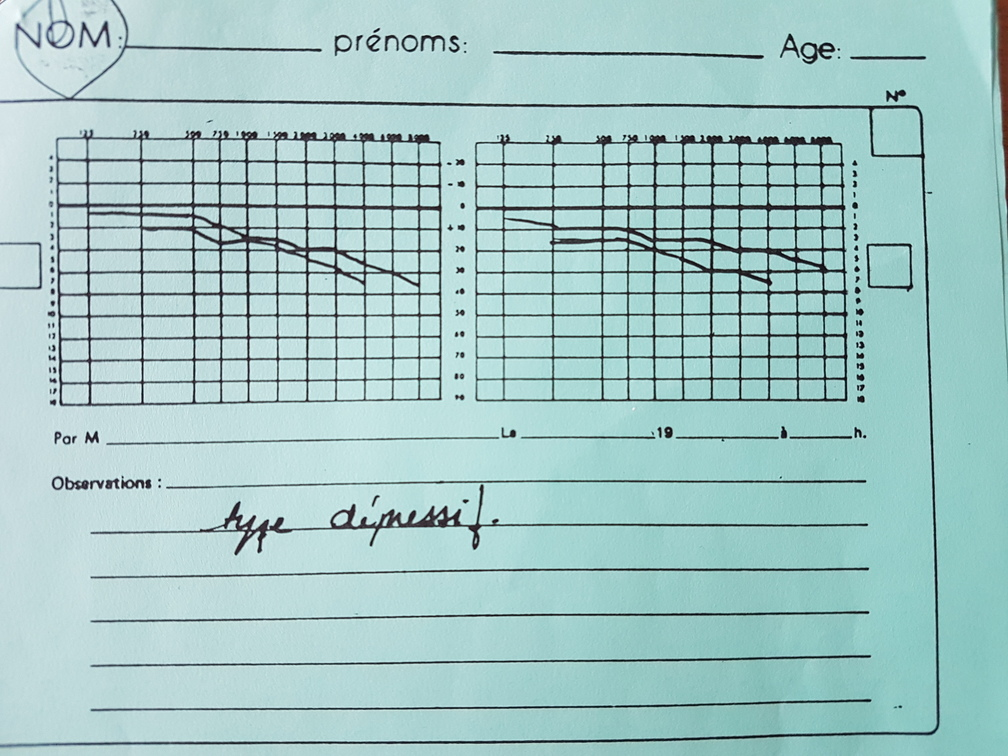
\includegraphics[width=0.7\linewidth]{images/courbedepressif.jpg}
                            %	\caption[Exemple d'une courbe de dépressif]{Courbe
                             %         représentative d'un dépressif, extrait de l'étude de Nantes,
                               %      1987.}

                            %	\label{groupecontroleimage1}
                            %\end{figure}





                          

                       



                            %`\textit{`La mélodie est la seule forme musicale de la décharge individuelle,
                            %car le rythme est le moteur, pré-musical, et l'harmonie,
                            %supra-individuelle ``} (Mosonyi, 1835????, cité par Michel, 1965).


                           % Ainsi, au lieu de séparer les trois grandes voies de la psychologie du
                            %XXème siècle (psychanalyse, comportementalisme et pychologie
                           % humaniste)
                            %\autocite[197]{van_eersel_cerveau}, il serait intéressant et important de les
                           % considérer comme complémentaires.
                            %, comportant chacun un aspect qu'il
                            %nomme ``phénomène humain''.











%Nous avons utilisé un type de test d'écoute dont nous soulignons la
%complexité du test d'écoute utilisé.%, puisant
%à la fois ses racines dans l'audiologie et à la fois dans la psychologie.
%Par celui-ci, nous voyons
%qu'il  existe une possible transformation
%individuelle lors d'une
%thérapie tout
% en constatant une forme de singularité pour chacun et une
%certaine similarité selon certaines pathologies. --Comme nous l'avons
%constaté avec l'étude J.P.Granier... il existe des points communs lors des recueils des seuils
%auditifs--.

%Nos résultats
%principaux sont les suivants:

%le groupe de musicothérapie a démontré une réactivité très positive
%dans son écoute par comparaison pré/post-thérapies tandis que
%le groupe de contrôle n'a démontré qu'une très faible
%modification dans son écoute.
%Il existe ainsi une différence importante entre les résultats des
%deux groupes.

%Il convient à présent de discuter des aspects énoncés (test et
%mesures),  puis des
%limites et perspectives.
%et les résultats obtenus.

%, en  éveille tout au
%moins cette idée, un déclenchement de travail initié tel un début de cheminement.
%Être accompagné dans la lecture de son évolution par le biais de
%son écoute
%est une façon différente d'entrevoir sa problématique. Elle permet de
%constater un résultat qui  peut le conforter ou non dans son sentiment
%intérieur.

%Il en est de même pour la simultanéité des
%résultats et le décalage intérieur vécu.

%quand donc il y a t il une fin dans une thérapie??)

%car le temps jouant son rôle, les étapes ne peuvent être brûlées. %avec différentes étapes --acceptation, refus, que
%ce soit au sujet de  son
%identité, de sa transformation--.
%car quitter le ``confort'' de ses habitudes, même d'écoute, peut être très perturbant, dérangeant.


%le patient est toujours en
%attente des résultats,comme un score à atteindre, impatient d'un résultat visible,
%avec la volonté ferme d'acquérir la courbe dite ``idéale'', n'écoutant pas son
%sentiment intérieur car trop sensible aux notions de performance,
%le test, de manière générale, peut être complètement
%contradictoire et totalement inapproprié.

% Changer de rail, être
%sur un quai de gare
%en attente d'un autre train, peut être vécu sous l'emprise de la
%panique ou la joie de l'inconnu.

%suggérées par une modification d'écoute.

%Quitter le confort même si elles sont jugées négatives par lui-même et par les autres --- . Tout ceci prend du temps et ne peut pas


%\textbf{ Auto-critique }


  %une hétéro-évaluation par un proche
  %aurait pu être pertinente.

%Par cette démarche, nos sommes conscients qu'il y a un risque de
%catégoriser le patient par les  transmis
%aux assurances-maladies.


%entr'autres la réintégration progressive de la voix  dans
%le corps.
%\footnote{ la correction de
%la voix se fait chez Tomatis grâce à des écouteurs spécifiques, incitant à
%l'émettre en retour }.
%la découverte ou redécouverte de ses ressources,
%la régénération énergétique, en définitive, la capacité d'être auteur de sa propre
%restructuration et \textbf{chef d'orchestre de sa
%vie.}\footnote{Jean-Pierre Granier, Tomatis
%Développement,\emph{Conférence Paris lors de la Convention du 13 mai
%2012}, 13.5.2012.}%


  % En comparaison avec des
  %modifications importantes de courbes des tests observées généralement  lors d' une écoute
  %régulière de deux heures par jour de musique pendant 15 jours --- en
  %référence à l'entrainement des muscles de l'oreille chez Tomatis,
  %qui, nous le rappelons, est une pédagogie de l'écoute --- il aurait
  %été intéressant de pouvoir faire cette étude comparative dans cette
 % clinique. Ainsi, nous aurions pu éventuellement mettre en avant
 % l'absolue nécessité de
  %Créer et d'instaurer systématiquement la
  %%musicothérapie dans de nombreuses institutions,
  %la développer beaucoup plus intensément, plusieurs fois par semaine.
    % Le patient reste au centre de nos préoccupations.
%Serait-ce une façon de démontrer l'utilité de la musicothérapie
%pour une plus large acceptation de
%cette thérapie dans plus de milieux hospitaliers ou autres ?
%, avec les
%nouveautés en neuroscience et en neuropsychologie sur les musies, les
%fonctions musicales du cerveau en les reliant avec les Muses.




 %Perspectives musicales futures: le 1° Symposium
  %NeuroTechSymphony, une première en Europe, a eu lieu au CHUV le 18 et 19 septembre 2019. Il  nous a
  %donné un aperçu de l'ampleur de la grande avancée technologique
  %%et de l'émergeance entre  l'interface de la musique, la technologie, la
  %création de jeux interactifs spécifiques avec leur fort impact sur la
  %réhabilitation. Nous avons aussi suivi avec intérêt l'étude en cours avec utilisation de
 % Biomarkers en Neuromusicology par le Prof. Artur Jaschke sur des
 % bébés prématurés prouvant l'effet de la musique ``en live'' sur leur
  %oxygénation, et donc sur leur diminution de stress.










\chapter{ Conclusion }

%\textbf{Le rôle primordial de l'oreille:}

%"Empathisches Zuhören ist eine unabdingbare Voraussetzung für empathisches Verstehen“ 
%\autocite[p.46]{seminar_zuerich} Eckert (2007)
%\textit{"L'écoute empathique est une condition indispensable
%	pour une compréhension empathique"}\footnote{traduction libre}.
Nous avons souligné dans notre travail le rôle primordial de
l'oreille. % qui "..est l'organe le plus sensible des
%sens et l'instrument de diagnostic le plus important du
%musicothérapeute'' pour ``\textit{rester en contact émotionnel}'' par le \textbf{son} qui va au plus 
%\%textbf{profond de
%	l'être} nous dit Eckert.
%Elle se dresse, \autocite {seminar_zuerich}, pour une\textbf{ écoute} empathique, pour ``\textit{rester 
%en contact émotionnel}'' par le \textbf{son} qui va au plus \textbf{profond de
%  l'être}. 
Ce que nous pouvons constater lors de l'aboutissement
d'une thérapie n'est pas le surgissement d'une autre personne mais une transformation
de la perception de celle-ci par rapport à elle-même et au monde qui l'entoure.
Être au diapason, en harmonie avec soi et les autres, nécessite une capacité d'écoute apte à nous 
accorder avec l'univers, avec un \enquote {consentement cellulaire}, comme nous le 
confiait cette patiente.

Vivant dans un monde très visuel, les preuves doivent être
validées pour soutenir l'argumentation du bien-fondé d'une thérapie
\autocite{vrait_musicotherapie_2018}.
     % On veut voir pour croire.
%Notre esprit formaté par le cartésianisme depuis bien longtemps nous
%empêche de penser différemment
%Actuellement, c'est une nécessité due à notre époque pour
%et nous mène à vouloir constamment crédibiliser l'impact
%du \textbf{son} sur notre être.
%Malgré l'immense progrès que l'IRMf a apporté à la musicothérapie, 
Nous restons
  ligotés par notre esprit occidental, par
  notre pensée analytique et linéaire, à la recherche de
  causes afin de crédibiliser l'impact
  du \textbf{son} sur notre être.
  D'après Janssen,\autocite{van_eersel_cerveau}, depuis Aristote, la modernité et le
siècle des Lumières, le postulat demeure de se positionner en dehors
de la nature, d'analyser, d'observer.
Rester sur ce plan, malgré les
indéniables résultats, est néanmoins
réducteur.
La musicothérapie  se retrouverait actuellement
 à un tournant décisif où elle est reconnue comme étant \textbf{intégrative} 
 \autocite{vrait_musicotherapie_2018},
struc\-tu\-rale, dans le sens où elle permet un travail d'élaboration psychique dans une perspective de structuration identitaire  et dans celui de l'intégration des données neuroscientifiques.
\textit{"Appréhender un phénomène vivant, qui est intégratif en soi, demande un esprit
  intégratif''} \autocite[201]{van_eersel_cerveau}.
Il est toutefois périlleux d'utiliser en soi un outil analytique -- tel s'est efforcé néanmoins ce travail -- et
plus
particulièrement en musicothérapie, où l'intuition, 
considérée comme un \textit{``phénomène intégratif ''}, reste essentielle.
%Comme l'exprime si justement Christophe André \autocite[154]{van_eersel_cerveau},

%Ainsi, même si le renfort d'études
%scientifiques est irremplaçable, le travail avec le patient, guidé plus par des résultats
%concrets que par des théories, se représentera toujours
%tel un
%explorateur du XVème siècle navigant sur des flots inconnus et
%s'engageant sur d'autres terres.


%\emph{"Le monde de	l'art n'est pas celui de l'immortalité, c'est celui de la
%        métamorphose."}     André Malraux.
 %    De même, la musique est un art produit par l'homme et qui a un impact
%sur lui-même. Les deux interagissent, s'interpénètrent et s'auto-transforment
%au cours des siècles.
%\begin{quotation}
%\emph{<<\,\emph{Par le Son, le Silence du Non-Être vient à l'Être}. [\dots]
%\textsl{Je suis}
%	\emph{la musique que je fais ou écoute}. [\dots]\,>>
%[\ldots] \emph{la musique a la capacité d'harmoniser
%les composantes d'une entité psychophysique pour qu'il soit ``bien
%dans sa peau'' et ``bien dans son âme}''}.\, \autocite[p.8]{viret:b}
%\end{quotation}
Ainsi nous resterons des explorateurs navigant sur des flots inconnus et
s'engageant sur d'autres terres.
Nous faisons partie d'un Tout, nous ne sommes que poussière d'étoile,
nous sommes
\textit{\textbf{``les descendants de la  cristallisation de la musique primordiale de
l'univers''}} \autocite{delbaz_recherche_2016}\footnote{David Elbaz, astrophysicien, chef de laboratoire 
au CEA et Alain
Destexhe, chercheur en neurosciences intégratives et computationnelles
à l'Institut  NeuroPsi de Paris Saclay}.




      \begin{figure}[tbh]
        \centering
        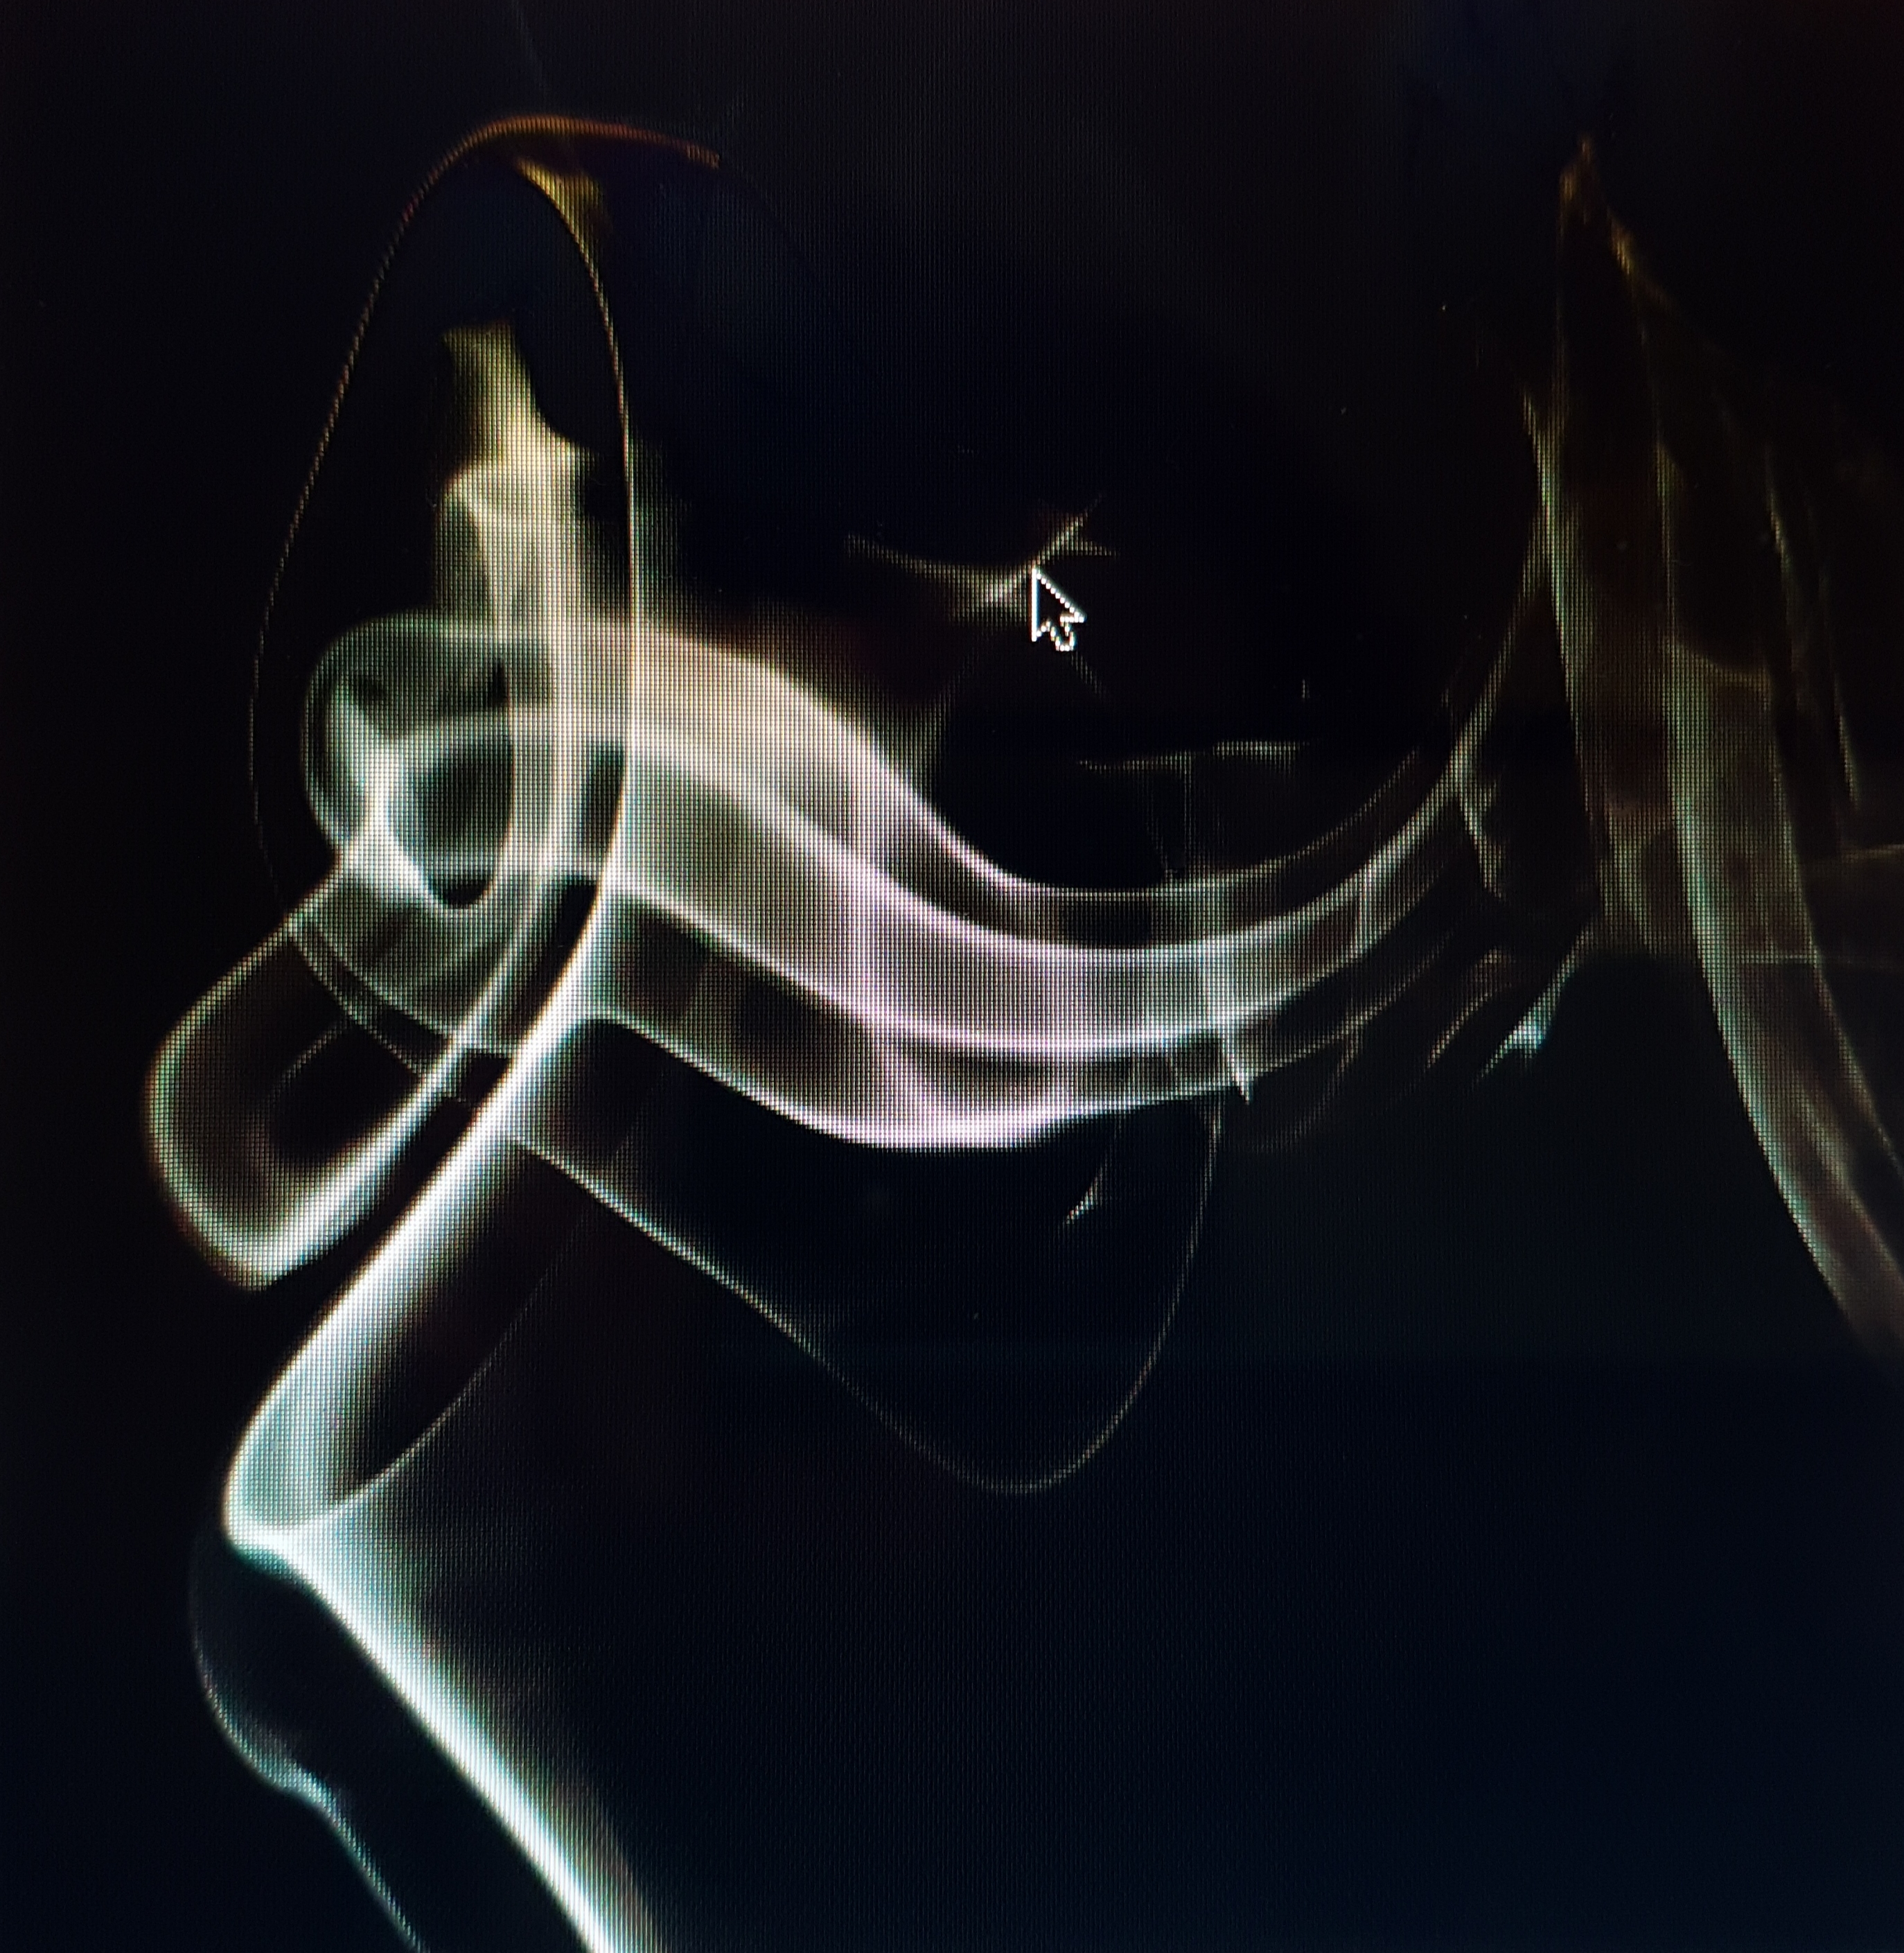
\includegraphics[width=1\linewidth]{images/oreillephoto.jpg}
        \caption{La Croche Oreille: plongée acoustique; EightBitTony, « Ear», Creative Commons by-nc.}
        \label{fig}
      \end{figure}


-----------------------------------------------------------------







%\textbf{Remerciements}


%A mes fils, Ambroise Lancelot, Arsène Eliott et Dorian Philéas, pour leur aide, soutien, patience et 
%compréhension tout au long de l'élaboration de ce travail.

%A Reto Rampa, directeur de mémoire,
%pour m'avoir donné confiance grâce à ses conseils
%avisés, et sa façon très subtile d'amener à la réflexion dans l'essentiel.

%A Regula Lehman, musicothérapeute à la Privatklinik von Meiringen pour sa présence affectueuse et 
%son aide précieuse dans l'organisation et planification des patients.

%%A Eva Hänni-Risler, Leiterin Therapeutische Dienste à la Privatklinik von Meiringen qui a donné son 
%%accord avec celui de la direction pour ce travail.

%A tous les patients qui m'ont permis de réaliser ce travail dans un climat de compréhension et un esprit 
%de curiosité et d'ouverture.

%A mon amie Fabienne, neuropsychologue à la SUVA, pour ses remarques pertinentes et ses encouragements.

%A mon frère Olivier, pour sa patience et aide dans les dédales des méandres de l'informatique.

%A Victoria, confidente de longue date, pour son indéfectible soutien.

%A Véronique, mon amie, cousine, avec sa bon humeur, son esprit vif et positif dans un formidable soutien.

%A Christine, mon amie flûtiste retrouvée aux hasards de la musique, à Sandrine, l'amie de toujours, à l'écoute, à Naomi et Octavia avec leur sensibilité et profondeur dans leur art de la danse, à toutes mes amies et amis, Alexandra, Chiara, Isabelle, Bernadette et leurs rires avec tant d'autres.

%A mon ami Bruno...et son humour.% et son éternelle présence dans l'absence...et son humour.

%A Laurent Tixier, le troubadour écrivain des temps nouveaux, avec sa douce Fanny, les vrais amis musiciens du bord de l'océan.

%A mes parents et grands-parents, au-delà du temps.

 %pulvérise le temps et l'espace.
%\end{Remerciements}




%Vivant dans un monde très visuel, les preuves sont
%validées pour soutenir l'argumentation du bien-fondé d'une thérapie
%\autocite[ch. II, pp. 105--106 ]{vrait_musicotherapie_2018}.
    %  On veut voir pour croire.
%Est-ce notre esprit formaté cartésien depuis quelques centaines d'années qui nous
%empêche de penser différemment
%Actuellement, c'est une nécessité due à notre époque pour
%t nous mène à vouloir toujours crédibiliser l'impact
%du \textbf{son} sur notre être?
%%%Malgré l'immense progrès que l'IRMf nous a apporté, nous restons
  %ligotés dans les preuves exigées par notre esprit occidental, dûes à
  %notre pensée analytique et linéaire, à la recherche de
  %causes.
%siècle des Lumières, le postulat demeure de se positionner en dehors
%indéniables résultats, est néanmoins
%réductionniste. Et
%  intégratif''} \autocite[201]{van_eersel_cerveau}.
%plus
%particulièrement en musicothérapie, où l'intuition reste essentielle,
%car le musicothérapeute étant un être
%extrêment sensible avec de multiples ``antennes'' utilise l'intuition.
%considérée comme un \textit{``phénomène intégratif ``}.

%primordial partie
%intégrante de
% l'écoute.
%  La musicothérapie fait partie de ces thérapies dites subtiles. Elle
%est très difficilement quantifiable. La
%psychologie cognitivo-comportementaliste peut le faire avec des
%tests.

%Certains  intégrent plus que d'autres dans leur pratique des techniques relevant du domaine de la psychothérapie--de l' analytique,
%  du comportementalisme, du cognitivisme, de la  systémique ainsi que
%  celles dites humanistes.  Le concept de \textit{"médium malléable"} a été
 % développé par  R.Rousillon\footnote{R.Rousillon,\textit{Paradoxes et situations li%mites,
  %%		de la psychanalyse} Paris, Puf. 1991}
  %et qu'il est possible de transposer dans la matière \textit{musique}
  %pour\textit{ `''favoriser et accompagner le processus
  %  de symbolisation''}
  %\footnote{F.X.Vrait, \textit{La musicothérapie},Ch.3, p. 112}.


%Ainsi Eckert \autocite{seminar_zuerich}\footnote{Eckert (2007)% definiert dieses folgendermaßen:„Um das Erleben des anderen wirklich verstehen zu können, muss man dem anderen zunächst einmal zuhören, und zwar so, dass man das, was der andere gesagt hat, vollständig und korrekt wiedergeben kann.
  %[...] Empathisches Zuhören ist eine unabdingbare Voraussetzung für empathisches Verstehen“ (S. 46)} souligne que l'\textbf{oreille }se dresse pour une\textbf{ écoute} empathique, pour ``\textit{rester en contact émotionnel}'' par le \textbf{son} qui va au plus \textbf{profond de
%  l'être}.


%Ce que nous pouvons constater lors de l'aboutissement
%d'une thérapie n'est pas de trouver une autre personne mais une transformation
%de la perception de celle-ci par rapport au monde qui l'entoure.


%\enquote{\emph{Le monde de
	%l'art n'est pas celui de l'immortalité, c'est celui de la métamorphose.}}
%nous rappelle André Malraux. De même, la musique est un art produit par l'homme et qui a un impact
%sur lui-même. Les deux interagissent, s'interpénètrent et s'auto-transforment
%au cours des siècles.




%Selon
%ce que nous vivons, nous nous transformons et continuons à être
%soi. Nous ``sommes soi" mais autrement. Nous ne perdons
%pas notre identité.



%Il n'y a
%amais, à proprement parler, d'avant et d'après mais il y a transformation.
%Et les transformations échappent toujours aux quantifications.

%Peut-être
%ici pourrons-nous apporter un outil plus objectif: la démonstration d'un travail d'écoute, d'une perception
%différente, d'une sensibilité nouvelle du patient.




% % Tomatis,utilisation de l'intuition de Tomatis comme Rogers(
% cf. ch. l'approche de C.Rogers dans Nicolas Duruz, Traité  des
%  psychothérapies comparées.

%Apprendre à écouter,
%c'est un travail et des résultats pourraient être visibles.




%Dans la même lancée, et déjà pressenti et  pensé au début de notre travail, Viret
%est de l'idée que\label{jeSuisLaMusique:viret}
%\begin{quotation}
%\emph{<<\,\emph{Par le Son, le Silence du Non-Être vient à l'Être}. [\dots]
%\textsl{Je suis}
%	\emph{la musique que je fais ou écoute}. [\dots]\,>>
%[\ldots] \emph{la musique a la capacité d'harmoniser
%les composantes d'une entité psychophysique pour qu'il soit ``bien
%dans sa peau'' et ``bien dans son âme}''}.\, \autocite[ch. 1, p.8]{viret:b}
%Être au diapason, en harmonie avec soi et les autres,
%nécessite une\textbf{ écoute } afin de nous accorder ou réaccorder à
%l'univers, et, comme l'exprime si poétiquement David Elbaz, nous
%sommes tous


%\textit{\textbf{``les descendants de la  cristallisation de la musique primordiale de
%l'univers''}} \autocite{delbaz_recherche_2016} \footnote{David Elbaz, astrophysicien, chef de laboratoire au CEA et Alain
%Destexhe, chercheur en neurosciences intégratives et computationnelles
%à l'Institut  NeuroPsi de Paris Saclay}.













%Réflexion:
%Concernant Ch.Tomatis p.39 et p.57, p.65, p.60 et suite, nous nous penchions sur les
%aspects interprétatifs, l'herméneutique appliquée aux connaissances
%neuropsychologqiues actuelles, associée à une approche holistique
%tenant compte aussi des aspects socio-psycho-culturels et systémiques.

%il serait intéressant et souhaitable de confronter les différentes fonctions des 3
%zones mentionnées avec les connaissances actuelles de la
%neuropsychologie au niveau des fonctions inférieures et supérieures.
%Les noyaux (reptilien, végétative) =inférieur avec la complexification
%des fonctions supérieures.
%Botez et Peretz, A. et H. Damasio
%Les conditions de maturation ont beaucoup changé avec la société que
%les découvertes de Tomatis mériteraient d'être réélaborées et
%reconsidérées.
%Le courant Tomatis pourrait être remise à jour grâce à J.P.Granier,
%Auriol ; comment évoluent les théories de Tomatis ( nouveautés et
%qu'est-ce qui a perdu de valeur = bilan général? entre le passé et le
%présent et le futur)
%Qu'est-ce qui a changé? la balance à plusieurs bras, elle se penche
%plutôt sur les aspects nouveaux, malgré le coût cher, l'intérêt se
%porte sur la neuropsychologie de la musique, y compris les dynamiques
%groupales.

%Grâce à ce travail, on peut se rendre compte qu'il y a des horizons beauccoup
%plus lointains qui apparaissent.

%Séminaire ...Monsieur ,,,et ...m'ont encouragé à persister dans cette voie
%méritent d'être mentionné comme modèle de forces rénovatrices,
%entr'autres les miennes.



%Pour élargir le concept de\textbf{ la zone 3,} comme on le
%verra dans la rubrique des réflexions, nous pourrions
%également l'étendre aux notions winnicottiennes du jeu, de la capacité
%créative dans un espace
%intermédiaire, où l' \textit{``objet
%transitionnel'' } (développé dans \textit{``Jeu et Réalité'',1953})
%figure entre le ``le
%dedans et le
%dehors'',
%l'interne et l'externe, et de là,  prolonger le questionnement du
%rapport avec le concept des
%courbes aérienne et osseuse.




%Peut-être pouvons-nous nous imaginer que la technologie future apportera d'autres outils
%directement accessibles pendant les séances, afin
% de, si nécessaire, visualiser directement l'effet en temps réel de la musique sur le
% cerveau:  imager couramment et facilement la manière d'ouïr de chaque
 %patient peut se révéler important, complémentaire et intéressant pour
 %l'anamnèse et la prise en charge. Ce serait l'image de la
 %physiologie de l'audition personnalisée à chaque séance!


%Nous sommes tout à fait conscients des
 %grandes divergences d'opinions entre les adeptes d'une musicothérapie
 %traditionnelle et cette méthode.
%Ce sont des concepts très différents. Bien que la notion d'écoute les réunit, bien que leur medium soit la musique et plus particulièrement le son, d'un côté il s'agit d'une thérapie et de l'autre, il s'agit d'une pédagogie, d'un entrainement de la musculature de l'oreille.
%Tomatis se focalise et opère essentiellement sur le capteur auditif
%(vestibulo-cochléaire) pour amener, par ce processus, le patient à une
%certaine  amélioration par rapport à sa vie actuelle et à des attentes
%précises. % cette amélioration peut se réaliser aussi au niveau du
%langage et ce, par l'intermédiaire de la musique et du chant.
%Avec le travail dit\textbf{ passif}, le  but est l'\emph{ouverture} de l'oreille
%aux sons et sa sensibilisation car l'objectif est de réintégrer
%des fréquences perdues ou annihilées inconsciemment.
%Cette technique de travail amène un résultat
%physiologique, dérange les habitudes d'écoute pour faire agir
%et ré-agir le patient, en étant parfois pertubatrice jusqu'à provoquer
%un phénomène de rejet.
 %Avec le travail \textbf{actif}, on corrige la voix grâce à des écouteurs spécifiques
%car la correction de la voix y est instantanée et instaure les bons
%réflexes de la boucle audio-vocale. Puisque ce processus incite à
%assimiler et à analyser l'information sonore pour l'ajuster et
%l'émettre en retour,%Le patient
%analyse cette boucle permanente entre l'écoute et l'émission vocale
%afin de créer des réflexes sur lesquels il peut ``s'asseoir''

%nous pourrions émettre la supposition suivante: lorsque cette boucle
%phono-auditive est bien élaborée et installée, interviendrait très judicieusement le
%rôle éminemment important de la musicothérapie. L'oreille est
%prête, entraînée et apte à se transformer encore plus en profondeur, notamment sur le
%plan psychique. % avec tous les
%riches moyens proposés par la musicothérapie.
%C'est une préparation de terrain, un travail physique de
%fond, un entraînement de l'oreille pour que celle-ci soit totalement
% opérationnelle, prête à approfondir sur de nombreux plans
 %La première phase peut être considérée comme une étape pédagogique et
 %préparatoire afin que la
% \textbf{musicothérapie} puisse jouer ensuite pleinement son rôle, dont
 %ne serait-ce que d'accepter d'entendre sa
%propre voix.
%Le soutien du thérapeute est nécessaire pour permettre
%au patient de franchir cette étape.
%la poursuite de la réintégration progressive de la voix dans
%le corps, la découverte ou redécouverte de ses ressources,
%la régénération énergétique, la capacité d'être auteur de sa propre
%restructuration et chef d'orchestre de sa
%vie.


%Relevons le paradoxe de l'empreinte vocale obtenue sur l'écran d'un
%même sujet avec le même mot en s'efforçant de le faire de manière
%identique; ce qui prouve que chaque phonation est unique. Est-ce alors
%possible de l'analyser?cf.p.104 "la thérapie par les sons"





%simplement pour se
%sentir bien sa peau, bien dans son âme.
%Voilà l'hypothèse énoncée et ce que nous nous pouvons conclure, en effet.

%Perspectives et rétrospectives
%politiciens musicothérapeutes
%jamais oublier la cosmogonie grecque, le mythe, Orphée,
%progrès qui  ont été fait




%L'écoute est-elle unive
%rselle ou diférente selon l'individu?
% Même si chaque être humain semble constitué comme son prochain, en
 %observant de près nos empreintes digitales, on s'aperçoit de l'unicité
 %de chaque être. De même, chaque oreille est particulière, singulière
 %quoique physiquement identique et\textbf{ s'ouvre différemment à l'écoute par l'imprégnation
% aux expériences de la vie}, par le temps qui infuse des changements dans
 %notre être intérieur et extérieur. Nous sommes vivants dans nos
 %mouvements psychiques et physiques. Des traces en sont
% visibles dans l' écoute constamment  façonnée par les
%ressentis, par l'environnement, et, plus brièvement décrit, par cette perméabilité au
 %changement, la rendant unique et évolutive.
